
\chapter{Local Arithmetic Theory of Forms of Higher Degree}\label{chap3} %%% chap3

AS\pageoriginale INDICATED BY the title, we shall apply the results of
the first two chapters to study the arithmetic of forms $f$ of higher
degree considered over local fields. Broadly speaking, many facts that
we shall discover do represent generalizations to the case when $f$
has degree greater than $2$, of earlier results; however, several
striking new aspects are thrown up, which, as is not surprising, could
not have been expected for quadratic forms. These will be recognised
clearly, as we proceed further.

\section{Three Functions: $F_{\Phi}$, $F^{\ast}_{\Phi}$,
  $Z_{\Phi}$}\label{chap3:sec1} %%% sec1 

We shall use the notation in Chapter II,
\S 1, with the modification that $X=K^{n}$ for a
local field $K$, $[x,y]=x_{1}y_{1}+\cdots+x_{n}y_{n}$ for
$x=(x_{1},\ldots,x_{n})$, $y=(y_{1},\ldots,y_{n})$ in $X$. We shall
use the standard $\psi$, so that the self-dual measure $|dx|$ becomes
the product of the usual measure on $K$. We choose a non-constant
polynomial $f(x)=f(x_{1},\ldots,x_{n})$ in $K[x_{1},\ldots,x_{n}]$,
since the case when $f$ is a constant, is trivial.

The following well-known lemma will be useful to establish the
continuity of a function that we shall define by means of an integral.

\begin{lemma*}
  Let $(X,dx)$ be a measure space, $T$ a metric space (or just separable
  at every point) and $f(x,t):X\times T\to \mathbb{C}$ be such that $f$
  is continuous in $t$ for any fixed $x$ and locally integrable in $x$
  for any fixed $t$ and, further, $|f(x,t)|\leq
  \varphi(x)$\pageoriginale for a $\varphi$ in $L^{1}(X,dx)$, for every
  $t$. Then $\int\limits_{X}f(x,t)dx$ defines a continuous function of $t$.
\end{lemma*}

\begin{proof}
  is immediate, in view of Lebesgue's theorem.
\end{proof}

\subsection{Definition of $Z_{\Phi}$}\label{chap3:sec1:subsec1} %%% subsec1.1

For $\omega\in \Omega_{+}(K^{\times})$
extended by continuity to $K$ and $\Phi\in\mathscr{S}(K)$, the integral
$$
Z_{\Phi}(\omega)=\int\limits_{X}\Phi(x)\omega(f(x))|dx|
$$
defines a holomorphic function on $\Omega_{+}(K^{\times})$; in fact, for
$$
0\leq \sigma(\omega)\leq \sigma_{2}<\infty,\quad
|\omega(f(x))|=|f(x)|^{\sigma(\omega)}_{K}<\max
(1,|f(x)|_{K})^{\sigma_{2}}
$$
and $\Phi(x)\max (1,|f(x)|_{K})^{\sigma_{2}}$ is in $L^{1}(X)$.

\subsection{Definition of $F^{\ast}_{\Phi}$}\label{chap3:sec1:subsec2} %%% subsec1.2

With $f$ in
$K[x_{1},\ldots,x_{n}]$ chosen above, we define, for any $\Phi$ in
$\varphi(X)$, the function $F^{\ast}_{\Phi}$ on $K$ by
$$
F^{\ast}_{\Phi}(i^{\ast})=\int\limits_{X}\Phi(x)\psi(i^{\ast}f(x))
|dx|\quad\text{for} \quad i^{\ast}\in K.
$$

Applying the lemma above to $f(x,t)=\Phi(x)\psi(tf(x))$ and
$\varphi(x)=|\Phi(x)|$ it follows that $F^{\ast}_{\Phi}$ is continuous
on $K$ (and indeed, bounded and uniformly continuous). The definition
of $F^{\ast}_{\Phi}$ is deceptively simple but it is a rather
difficult function to investigate.

\subsection{The Measure $|\theta_{i}|$}\label{chap3:sec1:subsec3} %%% subsec{1.3}

The {\em critical set} $C_{f}$ for $f$ is the set of points $a$ in $X$
at which the gradient grad $f$ of $f$ is $0$. If, therefore, we define
$U(i)=f^{-1}(i)\backslash C_{f}$ for $i\in K$, then $a$ is in $U(i)$
if and only if $a\in X$ satisfies $f(a)=i$ and further at least one
partial derivative of $f$, say $\dfrac{\partial f}{\partial x_{k}}$,
does not vanish at $a$. Since $f(x)=i$ on $U(i)$, we have the relation
$$
\dfrac{\partial f}{\partial x_{1}}dx_{1}+\cdots+\dfrac{\partial
  f}{\partial x_{n}}dx_{n}=0.
$$

Taking\pageoriginale the exterior product of both sides with the
$(n-2)$ - form $dx_{1}$ $\Lambda\ldots\Lambda
\hat{dx}_{j}\Lambda\ldots\Lambda
\hat{dx}_{k}\Lambda\ldots\Lambda dx_{n}$ (where
$\hat{\phantom{a}}$ indicates that the differentials $dx_{j}$,
$dx_{k}(j<k)$ have been omitted), we obtain 
\begin{multline*}
  (-1)^{j-1}\dfrac{\partial f}{\partial x_{j}}dx_{1}\Lambda\ldots\Lambda
  \hat{dx}_{k}\Lambda\ldots\Lambda dx_{n}+(-1)^{k-2}\\
  \frac{\partial f}{\partial
  x_{k}}dx_{1} \Lambda\ldots\Lambda \hat{dx}_{j}\Lambda
  \ldots\Lambda dx_{n}=0 
\end{multline*}
Thus $\theta_{i}(x)=(-1)^{k-1}\left(\dfrac{\partial f}{\partial
  x_{k}}\right)^{-1}dx_{1}\Lambda\ldots\Lambda\hat{dx}_{k}\Lambda\ldots\Lambda
dx_{n}|_{U(i)}$ is a well-defined non-vanishing regular $(n-1)$ - form
around $a\in U(i)$ and thereby giving rise to a global regular and
non-vanishing $(n-1)$ - form on $U(i)$; this is just ``the residue of
$(f(x)-i)^{-1}dx$ along $U(i)$'' and we denote it still by
$\theta_{i}$. Now $\theta_{i}$ induces on $U(i)$ a Borel measure
$|\theta_{i}|$ such that for every continuous function $\varphi$ on
$X$ with compact support disjoint with $C_{f}$, we have 
\begin{equation*}
  \int\limits_{X}\varphi(x)|dx|=\int\limits_{K}\left(\int\limits_{U(i)}
  \varphi|\theta_{i}|\right)|di|.\tag{72}\label{chap3:sec1:subsec3:eq72}
\end{equation*} 
Furthermore, for every such $\varphi$, the function $i\mapsto
\int\limits_{U(i)}\varphi|\theta_{i}|$ is continuous on $K$. The proof
depends on the implicit function theorem for $X$. Let us assume, after
re-ordering the subscripts if necessary, that the partial derivative
$\dfrac{\partial f}{\partial x_{n}}$ does not vanish at a given point
$a=(a_{1},\ldots,a_{n})$ in $U(i)$. Since 
$$
\dfrac{\partial(x_{1},\ldots,x_{n-1},f(x))}{\partial
  (x_{1},\ldots,x_{n-1},x_{n})}(a)=\frac{\partial f}{\partial
  x_{n}}(a)\neq 0,\text{ \ we may use \ } x_{1},\ldots,x_{n-1}, f(x)
$$
as local coordinates at $a$. If $x'=(x_{1},\ldots,x_{n-1})$ and
$a'=(a_{1},\ldots,a_{n-1})$, then, by the implicit function theorem,
there exists a convergent power-series $g(x',t)$ in $x'-a'$, $t-i$
with coefficients in $K$, such that, around $a$, $f(x)=t$ if and only
if $x_{n}=g(x',t)$. Applying a partition of unity, if necessary, we
may suppose that $\varphi$ has its support ``near $a$''. Then for $t$
close to $i$, we have, by the very\pageoriginale definition of
$|\theta_{i}|$, that
\begin{equation*}
  \int\limits_{U(t)}\varphi|\theta_{t}|=\int\limits_{K^{n-1}}
  \varphi(x',g(x',t)) \left|\frac{\partial
  f}{\partial  x_{n}}(x',g(x',t))\right|^{-1}_{K}|dx'|.
  \tag{73}\label{chap3:sec1:subsec3:eq73}  
\end{equation*}
The lemma stated at the beginning of \S 1 ensures that
the right hand side of (\ref{chap3:sec1:subsec3:eq73}) is continuous in $t$. Also, our
assertions are independent of the manner in which the partition of
unity is chosen. Now integration on $K$ gives
\begin{align*}
\int\limits_{K}\left(\int\limits_{U(t)}\varphi|\theta_{t}|\right)|dt|
&=
\int\limits_{K^{n}}\varphi(x',g(x',t))\left|\frac{\partial(x',x_{n})}{\partial
(x',t)}\right|_{K}|dx'|\;|dt|\\
&=\int\limits_{X}\varphi(x)|dx|
\end{align*}
implying (\ref{chap3:sec1:subsec3:eq72}).

\subsection{Definition of $F_{\Phi}$}\label{chap3:sec1:subsec4} %%%% subsec{1.4}

For the sake of simplicity, let us {\em assume}, in the sequel, that
$C_{f}\subset f^{-1}(0)$ (equivalently, $U(i)=f^{-1}(i)$ for every
$i\in K^{\times}$). If $f(x)$ is homogeneous and if the characteristic
of $K$ does not divide $m$, the degree of $f$, then this assumption is
fulfilled; in fact, for $a=(a_{1},\ldots,a_{n})\in C_{f}$, we have
$$
0=a_{1}\frac{\partial f}{\partial x_{1}}(a)+\cdots+a_{n}\frac{\partial
  f}{\partial x_{n}}(a)=mf(a)
$$
which is impossible unless $f(a)=0$. Our assumption is not serious
when the characteristic of $K$ is $0$; for, then, by a theorem of
Bertini, $C_{f}$ is contained in finitely many fibres $f^{-1}(i)$
which can be reduced, after applying a suitable partition of unity to
the situation where there is only one fibre and therefore (by
translation), we may assume without loss of generality that
$C_{f}\subset f^{-1}(0)$. For $i\in K^{\times}$, we define 
\begin{equation*}
  F_{\Phi}(i)=\int\limits_{U(i)}\Phi|\theta_{i}|.
  \tag{73}\label{chap3:sec1:subsec4:eq73} 
\end{equation*}\pageoriginale
Then if $\Phi$ has compact support disjoint with $C_{f}$, then we know
from above that $F_{\Phi}$ is continuous on $K^{\times}$; if, however,
$\Phi$ has compact support which is not disjoint with $C_{f}$, we may
apply a partition of unity to isolate points on our fibre and conclude
that $F_{\Phi}$ is continuous. Thus, at least for the case of
$p$-fields, the continuity of $F_{\Phi}$ is clear. However, if $K$ is
an $\mathbb{R}$-field and if $\Phi$ in $\mathscr{S}(X)$ does not have
compact support, even the convergence of the integral above is not
clear, not to speak of the continuity of $F_{\Phi}$. We therefore take
up the typical case $K=\mathbb{R}$ and show that the integral defining
$F_{\Phi}(i)$ is absolutely convergent for every $\Phi$ in
$\mathscr{S}(\mathbb{R}^{n})$ and further, that $F_{\Phi}$ is continuous
on $\mathbb{R}^{\times}$. We may assume after a translation, that
$C_{f}\subset f^{-1}(a)$ for some $a\neq 0$ and that $i=0$ in
(\ref{chap3:sec1:subsec4:eq73}). In order to prove the continuity of $F_{\Phi}$ at $i(=0)$,
it is enough to show that for any $\epsilon>0$, there exists
$r=r(\epsilon)>0$ ensuring that
\begin{equation*}
\int\limits_{f^{-1}(b),||x||\geq
  r}|\Phi|\;|\theta_{b}|<\epsilon\tag{74}\label{chap3:sec1:subsec4:eq74}
\end{equation*}
for every $b$ with $|b|\leq \rho<|a|$, where, for
$x=(x_{1},\ldots,x_{n}|\in X$,
$||x||=(x^{2}_{1}+\cdots+x^{2}_{n})^{1/2}$; the rest is clear from the
case of compact support. We now appeal to the following lemma due to
H\"ormander (\cite{Hor 1}): for any polynomial $P(x_{1},\ldots,x_{n})\in
\mathbb{R}[x_{1},\ldots,x_{n}]$, there exist constants $c$,
$\alpha>0$, $\beta \geq 0$, such that
$$
|P(x)|\geq c\cdot
\frac{\dis(x,V(P))^{\alpha}}{\max(1,||x||)^{\beta}}\text{ \ for  every
  \ } x=(x_{1},\ldots,x_{n})\in \mathbb{R}^{n} 
$$
where $V=V(P)$ is the variety of the real zeros of $P$ and $\dis(x,V)$
is the distance of\pageoriginale $x$ from the (closed) set $V$. The
critical set $C_{f}$ is precisely the set of common zeros of
$\dfrac{\partial f}{\partial x_{i}}(1\leq i\leq n)$ and hence the same
as $V(P_{0})$ for $P_{0}(x)=\sum\limits^{n}_{i=1}\left(\dfrac{\partial
  f}{\partial x_{i}}\right)^{2}$. We now assert that
\begin{equation*}
  \eta=\inf\limits_{\substack{x\\ |f(x)|\leq
      \rho}}\{\max(1,||x||)^{\gamma}P_{0}(x)^{1/2}\}>0
  \tag{75} \label{chap3:sec1:subsec4:eq75}  
\end{equation*}
for a constant $\gamma\geq 0$. By H\"ormander's inequality, we have
\begin{equation*}
P_{0}(x)\geq
c\frac{\dis(x,C_{f})^{\alpha}}{\max(1,||x||)^{\beta}}\text{ \ for
  every \ } x\in X.\tag{76}\label{chap3:sec1:subsec4:eq76}
\end{equation*}
We claim that (\ref{chap3:sec1:subsec4:eq75}) holds for
$\gamma=(1/2)((m-1)\alpha+\beta)$, 
$m$ being the degree of $f$. Otherwise, let $S$ be a sequence of
points $x$ with $|f(x)|\leq \rho$ such that 
$$
\lim\limits_{x\in S}\max (1,||x||)^{2\gamma}P_{0}(x)=0
$$
implying incidentally that $||x||\to\infty$. This means, in view of
(\ref{chap3:sec1:subsec4:eq76}), that
\begin{equation*}
\lim\limits_{x\in
  S}||x||^{(m-1)\alpha}(\dis(x,C_{f}))^{\alpha}<c^{-1}\cdot
\lim\limits_{x\in S}||x||^{2\gamma}P_{0}(x)=0
\tag{77}\label{chap3:sec1:subsec4:eq77}
\end{equation*}
We may, therefore, assume that $||x||\geq 1$ and $||x||^{m-1}\dis
(x,C_{f})\leq 1$ for every $x$ in $C_{f}$. On the other hand, for
every $x$, there exists $y=(y_{1},\ldots,y_{n})\in C_{f}$ such that
$||x-y||=\dis(x,C_{f})$ and we have
\begin{align*}
|f(y)-f(x)| &\leq
\sum^{m}_{k=1}\sum_{i_{1},\ldots,i_{k}}\frac{1}{k!}\left|\frac{\partial^{k}f(x)}{\partial
  x_{i_{1}}\ldots \partial x_{i_{k}}}(y_{i_{1}}-x_{i_{1}})\ldots
(y_{i_{k}}-x_{i_{k}})\right|\\
&\leq \sum^{m}_{k=1}c_{k}||x||^{m-k}||y-x||^{k}\text{ \ with constants
  \ } c_{k}\\
&\leq c'||x||^{m-1}||x-y||\text{ \  for a constant \ } c'\\
&\to 0\qquad \text{by \ref{chap3:sec1:subsec4:eq77}.}
\end{align*}
But\pageoriginale this contradicts
$$
|f(y)-f(x)|\geq |f(y)|-|f(x)|\geq |a|-\rho(>0),
$$
for every $x$ in $S$. Thus \ref{chap3:sec1:subsec4:eq75} is valid with the chosen
$\gamma$ and 
$$
f^{-1}([-\rho,\rho])\subset\bigcup^{n}_{k=1}W_{k}
$$
where $W_{k}=\{x\in X;\max(1,||x||)^{\gamma}\left|\dfrac{\partial
  f}{\partial x_{k}}(x)\right|\geq \eta/\sqrt{n}\}$; in other words,
on $f^{-1}([-\rho,\rho])$ at least one of the partial derivatives goes
to $0$ at most like $||x||^{-\gamma}$ and not too rapidly. On the
other hand, since $\Phi\in\mathscr{S}(\mathbb{R}^{n})$, there exists a
constant $c''>0$ such that for every $x=(x_{1},\ldots,x_{n})\in X$ and
correspondingly $x'=(x_{1},\ldots,\hat{x}_{k},\ldots,x_{n})$ in
$\mathbb{R}^{n-1}$ with $||x'||^{2}=||x||^{2}-x^{2}_{k}$, we have
$$
\max(1,||x'||)^{n}\max (1,||x||)^{\gamma+1}|\Phi(x)|<c''
$$
for $1\leq k\leq n$. Therefore, for the left hand side of
(\ref{chap3:sec1:subsec4:eq74}), we have the upper estimate
\begin{multline*}
  \sum^{n}_{k=1}\int\limits_{\substack{f^{-1}(b)\cap W_{k}\\ ||x||\geq
      r}}|\Phi(x)|\;|1/\frac{\partial f(x)}{\partial x_{k}}|\; |dx'|\\
  \leq \frac{\sqrt{\eta}}{\eta} \sum\limits^{n}_{k=1} 
  \int\limits_{\substack{f^{-1}(b)\cap
    W_{k}\\ ||x||\geq r}}\max (1,||x||)^{\gamma}|\Phi(x)|\;|dx'|\\
  \leq \frac{\sqrt{\eta}}{\eta}mnc''r^{-1}\int\limits_{\mathbb{R}^{n-1}}
  \max(1,||x'||)^{-n}|dx'|=\mathcal{O}(r^{-1}),
  \text{   as  } r \to\infty. 
\end{multline*}
This is sufficient to take care of the continuity of $F_{\Phi}$.

\subsection{The Relations Between $F_{\Phi}$, $F^{\ast}_{\Phi}$ and
  $Z_{\Phi}$}\label{chap3:sec1:subsec5} %%%%% subsec{1.5} 

If $\sigma(\omega)>0$, then, for $\Phi\in\mathscr{S}(K)$, we have, by
definition, 
\begin{align*}
Z_{\Phi}(\omega) &= \int\limits_{X\backslash
  f^{-1}(0)}\Phi(x)\omega(f(x))|dx|\tag{78}\label{chap3:sec1:subsec5:eq78}\\
&=
\int\limits_{K^{\times}}\left(\int\limits_{U(i)}\Phi|\theta_{i}|\right)\omega(i)|di|\\
&= M_{K}(m_{K}\omega_{1}F_{\Phi})(\omega), \text{ \ in a formal sense.}
\end{align*}\pageoriginale
For every $i^{\ast}$ in $K$, we have, on the other hand,
\begin{align*}
F^{\ast}_{\Phi}(i^{\ast}) &= \int\limits_{X\backslash
  f^{-1}(0)}\Phi(x)\psi(i^{\ast}f(x))|dx|,\text{ \ since \ }
f^{-1}(0)\text{ \ has measure 0,}\\
&=
\int\limits_{K^{\times}}\left(\int\limits_{U(i)}\Phi|\theta_{i}|\right)\psi(ii^{\ast})|di|\\
&= \int\limits_{K^{\times}}F_{\Phi}(i)\psi(ii^{\ast})|di|\\
&= \int\limits_{K}F_{\Phi}(i)\psi(ii^{\ast})|di|,\text{ \  extending
  \ } F_{\Phi} \text{ \  to \ } K.
\end{align*}
\ie $F^{\ast}_{\Phi}$ is just the Fourier transform
$(F_{\Phi})^{\ast}$ of $F_{\Phi}$.

We note that both the integrals considered above are absolutely
convergent:
\begin{align*}
& \int\limits_{K^{\times}}|F_{\Phi}(i)\omega(i)|\;|di|\; \leq
\int\limits_{X}|\Phi(x)|\; |f(x)|^{\sigma(\omega)}_{K}|dx|<\infty,\\
& \int\limits_{K^{\times}}|F_{\Phi}(i)\psi(ii^{\ast})|\; |di|\leq
\int\limits_{X}|\Phi(x)|\; |dx|<\infty
\end{align*}

\subsection{Statement of a Theorem}\label{chap3:sec1:subsec6} %%%% subsec{1.6}

We now state the first substantial theorem, in our theory, for forms
of higher degree.

\setcounter{theorem}{5}
\begin{theorem}\label{chap3:sec1:subsec6:thm6} %%% {thm1.6}
Suppose\pageoriginale that the characteristic of $K$ is $0$ and that
$C_{f}\subset f^{-1}(0)$. Then there exists a set of $\lambda$'s with
$\text{Re } \lambda>0$ such that $Z_{\Phi}$ is in $\mathscr{Z}$, $F_{\phi}$
is in $\omega^{-1}_{1}\mathscr{F}$ and $F^{\ast}_{\Phi}$ is in
$(\omega^{-1}_{1}\mathscr{F})^{\ast}$. In particular,
$Z_{\Phi}(\omega)$ defined by (\ref{chap3:sec1:subsec5:eq78}) has a meromorphic
continuation to the whole of $\Omega(K^{\times})$ and further,
$F_{\Phi}(i)$ (respectively $F^{\ast}_{\Phi}(i^{\ast})$) possesses an
asymptotic expansion as $|i|_{K}\to 0$ (respectively
$|i^{\ast}|_{K}\to \infty$). 
\end{theorem}

The major part of the proof of this theorem which will be given in the
next two sections, is to show that $Z_{\Phi}$ is in $\mathscr{Z}$;
once that is proved, it will follow that $F_{\Phi}$ is in
$\omega^{-1}_{1}\mathscr{F}$ and hence $F^{\ast}_{\Phi}$ in
$(\omega^{-1}_{1}\mathscr{F})^{\ast}$. Indeed, together with the
absolute convergence of the integral for $Z_{\Phi}(\omega)$ mentioned
above and the continuity of $F_{\Phi}$, the fact that $Z_{\Phi}$ is in
$\mathscr{Z}$ will enable us to apply the Fourier inversion theorem
and conclude that
$$
F_{\Phi}=m^{-1}_{K}\omega^{-1}_{1}M^{-1}(Z_{\Phi})
$$
The rest of the assertions of Theorem \ref{chap3:sec1:subsec6:thm6} now follows from
the theorems proved in Chapter I.

\begin{Remarks*}
\begin{enumerate}
\renewcommand{\labelenumi}{\theenumi)}
\item The assumption that $C_{f}\subset f^{-1}(0)$ in Theorem
  \ref{chap3:sec1:subsec6:thm6} cannot be dropped. Consider, for example, the case when
  $n=2$, $f(x)=1+x_{1}x_{2}$ and $\Phi$ is the characteristic function
  of $V=P^{e_{1}}\times P^{e_{2}}$ with $e_{1}$, $e_{2}$ in
  $\mathbb{Z}$ satisfying $e_{1}+e_{2}\geq 1$. Then
  $C_{f}=\{0\}\subset f^{-1}(1)$ and with our former notation,
\begin{align*}
Z_{\chi}(z) &= \int\limits_{V}\chi(1+x_{1}x_{2})|dx|\\
&= \sum\limits_{j\geq
  e_{1}}(1-q^{-1})\int\limits_{1+P^{j+e_{2}}}\chi(u)du\\
&= q^{-\max(e_{1}+e_{2},e_{\chi})}\\
&\neq 0
\end{align*}
for every $\chi$. This violates condition (2) defining
$\mathscr{Z}(\Omega(K^{\times}))$. 

\item If\pageoriginale $K$ has characteristic $p>0$, then the
  condition ``$p$ does 
  not divide the degree of $f$'' is necessary (although not
  sufficient) to ensure that $Z_{\Phi}$ is in $\mathscr{Z}$. Consider
  now, for example, the case when $n=1$, $f(x)=x^{p}$ and $\Phi$ is
  the characteristic function of $R$. Then, for $|z|<q^{1/p}$, we can
  show that
$$
Z_{\chi}(z)=
\begin{cases}
\frac{1-q^{-1}}{1-q^{-1}z^{p}} & \text{if \ } \chi^{p}=1\\
0 & \text{if \ } \chi^{p}\neq 1.
\end{cases}
$$
But the number of $\chi$ in $(R^{\ast})^{\ast}$ with $\chi^{p}=1$ is
infinite; in fact, for the finite group $R/(1+P^{pj})$ with $j\geq 1$,
the cardinality of the cokernel of the $p^{\text{th}}$ power map is
$q^{(p-1)j}$ and therefore, the number of $\chi$ in
$(R^{\ast})^{\ast}$ with $\chi^{p}=1$ and $e_{\chi}\leq pj$ is
$q^{(p-1)j}$. Again condition (2) in the definition of
$\mathscr{Z}$ is violated by $Z_{\Phi}$.
\end{enumerate}
\end{Remarks*}

\subsection{Gaussian Sums and Singular Series}\label{chap3:sec1:subsec7} %%%subsec{1.7}

For any $p$-field $K$ and $e\in\mathbb{Z}$, let us denote the $n$-fold
product $P^{e}\times\ldots\times P^{e}$ of $P^{e}$ by $(P^{e})^{(n)}$
and for $e=0$, $R^{(n)}$ by $X^{0}$. If $f(x)\in
R[x_{1},\ldots,x_{n}]$ and $\Phi$ is the characteristic function of
$X^{0}$, we simply write $F$, $F^{\ast}$, $Z$ instead of $F_{\Phi}$,
$F^{\ast}_{\Phi}$, $Z_{\Phi}$ respectively. Then, without any further
assumption on $f$, we have, for $i^{\ast}=\pi^{-e}u$ with $e\geq 0$ in
$\mathbb{Z}$ and $u$ in $R^{\ast}$, the following relation:
$$
F^{\ast}(i^{\ast})=q^{-ne}\sum_{\xi\mod P^{e}}\psi(i^{\ast}f(\xi))
$$
which is immediate on writing any $x\in X^{0}$ as $\xi+\pi^{e}y$ with
$\xi$ running over $X^{0}\mod(P^{e})^{(n)}$ and $y\in X^{0}$. The sum
over $\xi$ modulo $(P^{e})^{(n)}$ is usually called a {\em generalized
  Gaussian sum}. Although this relation is quite straightforward, the
interesting fact is that, once we accept Theorem
\ref{chap3:sec1:subsec6:thm6}, then we get
$$
q^{-ne}\sum_{\xi\mod
  P^{e}}\psi(i^{\ast}f(\xi))=\sum_{\lambda,m}a^{\sharp}_{\lambda,m} 
(ac(i^{\ast}))|i^{\ast}|^{-\lambda}_{K}(\log |i^{\ast}|_{K})^{m-1}
$$
$=$\pageoriginale a fixed linear combination of functions of the form
$$
\chi(ac(i^{\ast}))|i^{\ast}|^{-\lambda}_{K}(\log|i^{\ast}|_{K})^{m-1}
$$
{\em for all sufficiently large} $e=-\ord (i^{\ast})$. Such a ``stable
behaviour'' of a generalized Gaussian sum is quite remarkable.

We also recall that for $i$ in $R$,
$$
N_{e}(i)= \text{ \ the number of \ } \xi \mod P^{e} \text{ \ with \ }
f(\xi)\equiv i \pmod{P^{e}},
$$
also plays an important role in the classical theory. If $f$ is
homogeneous of degree $m$, $i$ is in $R\backslash\{0\}$ and the
characteristic of $K$ does not divide $m$, then we will see that
\begin{equation*}
q^{-(n-1)e}N_{e}(i) \text{ is independent of } e, \text{ for } e\geq 2
\ord (mi)+1.\tag{79}\label{chap3:sec1:subsec7:eq79}
\end{equation*}
Further, for $i\neq 0$ in $R$, we have the relation
\begin{align*}
F(i) &= \text{ the above ``stable quotient'' }
q^{-(n-1)e}N_{e}(i)\tag{80}\label{chap3:sec1:subsec7:eq80}\\
&= \lim\limits_{e\to \infty}q^{-(n-1)}e_{N_{e}(i)}
\end{align*}
which is known as the {\em ``singular series''} associated with $f$
and $i$. The proof of (\ref{chap3:sec1:subsec7:eq79}) is given in the
appendix to this chapter. However, if we assume that
$$
K \text{ has characteristic } 0 \text{ and } C_{f}\subset f^{-1}(0)
$$
then (even for $f$ not necessarily homogeneous) we can use Theorem
\ref{chap3:sec1:subsec6:thm6} to derive, at one stroke, the relations
(\ref{chap3:sec1:subsec7:eq79}) in 
perhaps a less precise form and (\ref{chap3:sec1:subsec7:eq80}). The proof is as
follows. In fact, the theorem implies that $F_{\Phi}$ and, in
particular, $F$ ($=F_{\Phi}$ for $\Phi=\varphi_{X^{0}}$) is in
$\omega^{-1}_{1}\mathscr{F}$ and hence, locally constant on
$K^{\times}$. Thus there exists $e>\ord(i)$ such that $F(t)=F(i)$ for
all $t\in i+P^{e}$. If now, we take $\varphi$ to be the\pageoriginale
characteristic function of the compact open set $X^{0}\cap
f^{-1}(i+P^{e})$, the right hand side of (\ref{chap3:sec1:subsec3:eq72}) is just
\begin{align*}
\int\limits_{K}\left(\int\limits_{U(t)}\varphi|\theta_{t}|\right)|dt|
&= \int\limits_{i+P^{e}}\left(\int\limits_{U(t)\cap
  X^{0}}|\theta_{t}|\right)|dt|\\
&= \int\limits_{i+P^{e}}F(t)|dt|\text{ \ by definition
  \ref{chap3:sec1:subsec4:eq73}}\\ 
&= F(i)q^{-e}, \text{ since } F \text{ is constant on } i+P^{e}.
\end{align*}
But the left hand side of (\ref{chap3:sec1:subsec3:eq72}) is merely
\begin{align*}
m(X^{0}\cap f^{-1}(i+P^{e})) &= m(\{\xi\in X^{0};f(\xi)\equiv i \pmod{
P^{e}}\})\\
&= N_{e}(i)\cdot m(\pi^{e}X^{0})\\
&= q^{-ne}N_{e}(i).
\end{align*}
Hence there exists $e>\ord(i)$ such that
$$
F(i)=N_{e}(i)/q^{(n-1)e}
$$
and this relation persists even if we replace $e$ by a larger integer.

\section{Preparations for the Proof of the ``Main
  Theorem''}\label{chap3:sec2} %%%%%{chap3:sec2}

\subsection{}\label{chap3:sec2:subsec1} %%%% subsec{2.1}

We shall prove the ``main theorem'' \ie Theorem \ref{chap3:sec1:subsec6:thm6}, only for
$p$-fields $K$ and merely give an outline of the proof when $K$ is an
$\mathbb{R}$-field. First we explain the concept of a resolution of
(the singularities of) the surface defined by $f(x)=0$ in a general
set-up.

Let $k$ be an arbitrary field, $X$ an (absolutely) irreducible
non-singular algebraic variety defined over $k$ and $D$, a positive
$k$-rational divisor of $X$. Then a\pageoriginale $k$-resolution
$$
h:Y\to X
$$
of $D$ is defined by the following three conditions:
\begin{enumerate}
\renewcommand{\theenumi}{\roman{enumi}}
\renewcommand{\labelenumi}{(\theenumi)}
\item $h$ is an everywhere regular birational map of an irreducible
  non-singular algebraic variety $Y$ to $X$, with both $Y$ and $h$
  defined over $k$, such that $h$ can be written as a product of
  monoidal transformations each with an irreducible non-singular
  centre;

\item $h^{-1}$ is regular and hence biregular, at every simple point
  $a$ of $D$; and 

\item for every $b$ in $Y$, all the irreducible components of
  $h^{\ast}(D)$ passing through $b$ are defined over the field $k(b)$
  and further are mutually transversal at $b$.
\end{enumerate}

Although this may appear to be much too general, we shall deal in our
applications only with the cases when $X$ is either an affine or a
projective space and $D$, the divisor defined by a polynomial. Also,
that part of condition (i) which requires $h$ to be a product of
monoidal transformations may be replaced by the weaker condition that
$h$ is ``projective'', if our immediate objective is only to prove
Theorem \ref{chap3:sec1:subsec6:thm6}. However, the full force of condition (i) will be
used only later on. It should also be remarked that the monoidal
transformations cannot, in general, be required to be defined over $k$
itself.

We also consider the following situation. Suppose $D'$ is the sum of
irreducible subvarieties of codimension $1$ in $X$ which are defined
over $k$ and further mutually transversal at every point of $X$; in
our applications, $D'$ will be either $0$ or irreducible (and
non-singular). Moreover, let condition (iii) above be satisfied with
$h^{\ast}(D+D')$ in place of $h^{\ast}(D)$. Then we say that $h$ is a
$k$-{\em resolution of $(D,D')$.} If $h$ is a $k$-resolution of
$(D,D')$, then $h$ is also a $K$-resolution of $(D,D')$\pageoriginale
for any extension field $K$ of $k$. Moreover, for any $k$-open subset
$U$ of $X$, if $Y_{U}=h^{-1}(U)$ and $D_{U}$ (respectively $D'_{U}$)
are the restrictions of $D$ (respectively $D'$) to $U$, then $h$ gives
rise to a $k$-resolution $Y_{U}\to U$ of $(D_{U},D'_{U})$. These
assertions are quite obvious. But what is important is that {\em a
  $k$-resolution of $(D,D')$ always exists, if $k$ has characteristic
  $0$;} and this is indeed a consequence of Hironaka's fundamental
theorem (\cite{Hir}).

\subsection{}\label{chap3:sec2:subsec2}%%% {2.2}

If $h$ is a $k$-resolution of $(D,D')$, then every irreducible
component of $h^{\ast}(D+D')$ is non-singular. Let $E$ be an
irreducible component of $h^{\ast}(D)$; then we have
$$
h^{\ast}(D)=\sum_{E}N_{E}\cdot E
$$
where the integer $N_{E}$ is defined as follows. If $b$ is any point
of $E$ and if $D$ is defined locally by the equation $g=0$ around
$a=h(b)$, then the multiplicity of $E$ in $g\circ h=0$ is denoted by
$N_{E}$; this does not depend on the choice of $b$ in $E$. We say that
the $k$-resolution $h$ is {\em tame} if the characteristic of $k$ does
not divide any $N_{E}$.

We need to define another component for our datum. Let us choose local
coordinates $x_{1},\ldots,x_{n}$ around $a$ in $X$ and local coordinates
$y_{1},\ldots$, $y_{n}$ around $b$ in $Y$. Then the multiplicity of $E$
in the local divisor defined by
$\dfrac{\partial(x_{1},\ldots,x_{n})}{\partial(y_{1},\ldots,y_{n})}=0$
depends only on $E$ and is denoted by $\nu_{E}-1$. We call the pair
$(N_{E},\nu_{E})$ the {\em numerical datum of $h$ along $E$.}

We observe that $\nu_{E}\geq 1$ and further, that $\nu_{E}=1$ if and
only if $h$ is biregular at every point of $E$ not contained in any
other component of $h^{\ast}(D)$. If $E_{1},E_{2},\ldots$ are the
irreducible components of $h^{\ast}(D)$ passing through any point $b$
of $Y$, then the cardinality of the set $\{E_{i}\}$ is at most equal
to the dimension $n$ of $X$. If\pageoriginale we rewrite the numerical
datum of $h$ along $E_{i}$ as $(N_{i},\nu_{i})$, then we call
$\{(N_{i},\nu_{i})\}_{i}$ the {\em numerical data of $h$ at $b$.}

Suppose that $K$ is an extension field of $k$ and $h:Y\to X$ is a
$k$-resolution of $(D,D')$ as above. For any $K$-rational point $b$ of
$Y$ (\ie for $b\in Y_{K}$), let $x_{1},\ldots,x_{n}$ be local
coordinates around $a=h(b)$ on $X$ which are defined over $k$ and let
$D$ be defined locally around a by the equation $g=0$. Further, let us
write $dx=dx_{1}\Lambda\ldots\Lambda dx_{n}$. We can then find local
coordinates $y_{1},\ldots,y_{n}$ around $b$ on $Y$ which are defined
over $K$ and satisfy $y_{1}(b)=\ldots=y_{n}(b)=0$, such that we have
\begin{align*}
& g\cdot h =\epsilon\prod_{i}y^{N_{i}}_{i}\\
& h^{\ast}(dx)=\eta\prod_{i}y_{i}^{\nu_{i}-1}\cdot
  dy\tag{81}\label{chap3:sec2:subsec2:eq81}
\end{align*}
around $b$, with functions $\epsilon$, $\eta$ on $Y$ that are defined
over $K$ and invertible in the local ring of $Y$ at $b$. If $K$ is a
local field, we shall write $X$, $Y,\ldots$ etc.\@ for $X_{K}$,
$Y_{K},\ldots$, consistent with our previous notation.

\subsection{An Example}\label{chap3:sec2:subsec3} %%% subsec{2.3}

Suppose that $k$ has characteristic $0$ and $D$ is an absolutely
irreducible curve containing the origin $0$, in a $k$-open subset $X$
of the affine plane; let $0$ be the only singular point of $D$ and
further, $D$ absolutely analytically irreducible at $0$. It is
well-known that there exists then a unique minimal $k$-resolution of
$D$. Let $E_{i},i=1,2,\ldots,I$ be the exceptional curve ``created''
at the stage of the $i^{\text{th}}$ quadratic transformation. (We
remark that such an ordering of the exceptional curves is used only
here). Then the graph of the function 
$$
\varphi(i)=\nu_{i}/N_{i}\text{ \ for \ } 1\leq i\leq 1
$$\pageoriginale
has been examined in our paper \cite{Igu 7}. In the first approximation,
the graph looks as in the following figure.

\begin{figure}[H]
  \centering{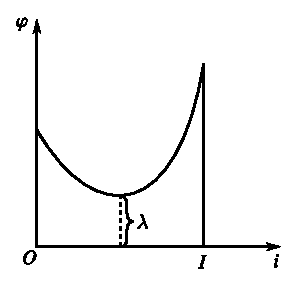
\includegraphics{fig59-1.eps}}
\end{figure}

The (strict) minimum value of $\varphi$, say $\lambda$, has a
remarkably simple meaning. If $f(x)=0$ is a local equation for $D$
around $0$ and $f_{m}(x)$ the leading form in $f(x)$, then after
replacing $x_{1}$ by $x_{1}+cx_{2}$ for some $c$ in $k$, if necessary,
we may suppose that $f_{m}(0,1)\neq 0$. Then we can solve the equation
$f(x)=0$ by a power-series $x_{2}=g(x_{1})$ in $x^{1/m}_{1}$. Let
$x^{r}_{1}$ be the first non-integral power of $x$ appearing in
$g(x_{1})$ with non-zero coefficient. Then the so-called ``first
characteristic exponent'' $r$ satisfies $r>1$ and further,
$$
\lambda=\frac{1}{m}\left(1+\frac{1}{r}\right).
$$
In particular, for $f(x)=x^{n}_{1}-x^{m}_{2}$ with $m$, $n$ coprime
and $1<m<n$, we have $r=n/m$ and hence,
$\lambda=\dfrac{1}{m}+\dfrac{1}{n}$.

\subsection{}\label{chap3:sec2:subsec4} %%% subsec{2.4}

The following lemma will prove useful later, for example, in settling
the rationality of $Z_{\Phi}(\omega)$.

\setcounter{lemma}{3}
\begin{lemma}\label{chap3:sec2:subsec4:lem4} %%% {lem2.4}
  For a $p$-filed $K$, let $\omega$ be in $\Omega(K^{\times})$ with
  $\omega(\pi^{i}u)=z^{i}\chi(u)$ as before and further, let
  $\nu+N\sigma(\omega)>0$ (or, equivalently $|q^{-\nu}z^{N}|<1$) for
  given $N$, $\nu$ in $\mathbb{Z}$. Then,\pageoriginale for any $c$ in
  $K$ and $e$ in $\mathbb{Z}$, we have 
   {\rm 
    \begin{multline*}
    \int\limits_{c+P^{e}}\omega(t)^{N}|t|^{\nu-1}_{K}|dt|=
     \begin{cases}
      (1-q^{-1})q^{-\nu e}z^{eN}/(1-q^{-\nu}z^{N})\\ 
      0\\ 
      \chi^{N}(c\pi^{-\ord(c)})q^{-(\nu-1)\ord(c)-e}z^{\ord(c)N} \\
      0  
    \end{cases}\\
      \begin{array}{l}
        \text{if }~ \chi^{N}  =1 \text{ and } c\in P^{e}\\
        \text{if }~ \chi^{N}  \neq 1\text{ and } c\in P^{e}\\
        \text{if }~ \chi^{N}  =1\text{ on } 1+c^{-1}P^{e}\text{ and }
        c\not\in P^{e}\\ 
        \text{if }~ \chi^{N}  \neq 1 \text{ on } 1+c^{-1}P^{e}\text{ and }
      c\not\in P^{e}
      \end{array} \tag{82}\label{chap3:sec2:subsec4:eq82}
  \end{multline*}}
\end{lemma}

\begin{proof}
  Let $e_{0}=\ord(c)$ and $u_{0}=c\pi^{-e}$. Then, for $c\in P^{e}$, the
  left hand side of (\ref{chap3:sec2:subsec4:eq82}) is clearly the same as
  \begin{multline*}
  \sum_{i\geq e}(q^{-\nu}z^{N})^{i}\int\limits_{R^{\times}}\chi^{N}(u)du=\\
  \begin{cases}
    (1-q^{-1})(q^{-\nu}z^{N})^{e}/(1-q^{-\nu}z^{N}) & \text{for }
    \chi^{N}=1\\
    0 & \text{if } \chi^{N} \text{ is non-trivial.}
  \end{cases}
  \end{multline*}
If, however, $c\not\in P^{e}$, then the left hand side of
(\ref{chap3:sec2:subsec4:eq82}) 
is obviously equal to
$\omega(c)^{N}|c|^{\nu}_{K}\int\limits_{1+c^{-1}P^{e}}\chi^{N}(u)du$
on applying $t\mapsto ct$ and this is then seen to coincide with the
expression on the right hand side.
\end{proof}

\subsection{}\label{chap3:sec2:subsec5}%%% subsec{2.5}

Let $m$ denote a positive integer and let us denote the map $x\mapsto
x^{m}$ in $K$ by $[m]$. Thus, for any subset $S$ of $K$, we have
$S^{[m]}=\{s^{m};s\in S\}$. The following lemma gives a very precise
description of the images under $[m]$ of certain subsets of $R^{\times}$
in a $p$-field $K$.

\begin{lemma}\label{chap3:sec2:subsec5:lem5} %%% {lem2.5}
  If $m$ is a natural number not divisible by the characteristic of a
  $p$-field $K$, then, for every integer $i>\ord(m)$, we have
  $$
  (1+P^{i})^{[m]}=1+mP^{i}.
  $$
\end{lemma}

\begin{proof}
  Our\pageoriginale proof depends on the following simple version of
  Hensel's lemma. For any $g(x)$ in $R[x_{1},\ldots,x_{n}]$ and $a$ in
  $X=K^{n}$, let $\mathscr{X}=\mathscr{X}(a)$ be defined by 
  $$
  \mathscr{X}=\mathscr{X}(a)=\min\left\{\ord \left(\frac{\partial
    g}{\partial x_{1}}(a)\right),\ldots,\ord\left(\frac{\partial
    g}{\partial x_{n}}(a)\right)\right\}
  $$
  so that $\mathscr{X}(a)=\infty$ if and only if $a$ is in $C_{f}$. {\em
    If for $a$ in $X^{0}\backslash C_{f}$, we have $g(a)\equiv 0(\mod
    P^{2\mathscr{X}+1})$, then there exists $b$ in $X^{0}$ such that}
  \begin{equation*}
    g(b)=0\text{ \textit{and} } b\equiv a \pmod{g(a)P^{-\mathscr{X}}}
    \tag{83}\label{chap3:sec2:subsec5:eq83} 
  \end{equation*}
      {\em In particular, every simple point $a\mod P$ on $g(x)\equiv 0\pmod{
        P}$ can be ``lifted'' to a point $b$ of the variety given by
        $g(x)=0$, in $X^{0}$.} For the sake of completeness, we give a quick
      proof of (\ref{chap3:sec2:subsec5:eq83}). If $e_{0}=\ord(g(a))$,
      then $e_{0}\geq 
      2\mathscr{X}+1$; let us exclude the trivial case when
      $e_{0}=\infty$. We can construct, as follows, a sequence
      $$
      a^{(0)}=a,\quad a^{(1)},\quad a^{(2)},\ldots
      $$
      in $X^{0}$ such that
      \begin{equation*}
      g(a^{(i)})\equiv 0\pmod{P^{e_{0}+i}}\text{ and } a^{(i)}\equiv
      a^{(i-1)} {\pmod{P^{e_{0}+i-1-\mathscr{X}}}}
      \tag{84}\label{chap3:sec2:subsec5:eq84} 
      \end{equation*}
      for $i\geq 1$. For $i=0$, the first condition in
      (\ref{chap3:sec2:subsec5:eq84}) is already
      true while the second condition is non-existent. Assume
      (\ref{chap3:sec2:subsec5:eq84}) to 
      have been proved for some $i\geq 0$ and set
      $$
      a^{(i+1)}=a^{(i)}+\pi^{e_{0}+i-\mathscr{X}}t
      $$
      with an unknown $t=(t_{1},\ldots,t_{n})$ in $X^{0}$. Then we have
      \begin{align*}
      g(a^{(i+1)}) & \equiv 0\pmod{P^{e_{0}+i+1}}\Leftrightarrow
      \sum^{n}_{k=1}\pi^{-\mathscr{X}}\frac{\partial g}{\partial
        x_{k}}(a)t_{k}\\
      & \equiv -\pi^{-(e_{0}+i)}g(a^{(i)})\pmod{P}
      \end{align*}
      in view of $e_{0}\geq 2\mathscr{X}+1$, on using the Taylor expansion
      of $f$. Now the definition of $\mathscr{X}$ enables us to establish
      \ref{chap3:sec2:subsec5:eq84} for $i+1$ instead of $i$
      and \ref{chap3:sec2:subsec5:eq83} follows from the
      completeness of $K$.
\end{proof}

We\pageoriginale proceed to derive Lemma \ref{chap3:sec2:subsec5:lem5}
from our version 
of Hensel's \break lemma. It is clear that, for $i\geq \ord(m)$, we have
$(1+P^{i})^{[m]}\subset 1+mP^{i}$. In order to prove the reverse
inclusion for $i>\ord(m)$, we have only to start from any element
$1+m\pi^{i}a$ of $1+mP^{i}$ with $a\in R$ and set
$$
g(x)=(m\pi^{i})^{-1}((1+\pi^{i}x)^{m}-(1+m\pi^{i}a))
$$
Then $g(x)\equiv x-a(\mod P)$ and $a \mod P$ is a simple point on
$g(x)\equiv 0(\mod P)$. Therefore, we have, from above, an element $b$
of $R$ with $g(b)=0$, proving the desired inclusion and the lemma.

\section{Proof of Theorem 1.6 for $p$-Fields}\label{chap3:sec3} %%%% {chap3-sec3}  

\subsection{Reformulation of the Theorem for
  $p$-Fields}\label{chap3:sec3:subsec1} %%% subsec{3.1}

Let $K$ be a $p$-field and then, by our identification of $X$, $Y$
etc. with $X_{K}$, $Y_{K}$ etc., $X$ is the same as $K^{n}$. Instead
of assuming that $C_{f}\subset f^{-1}(0)$, let us make the weaker
assumption that, for the given $\Phi$ in $\mathscr{S}(X)$, its support
$\Supp(\Phi)$ satisfies the condition
\begin{equation*}
C_{f}\cap \Supp\Phi\subset f^{-1}(0).\tag{85}\label{chap3:sec3:subsec1:eq85}
\end{equation*}
Let us recall that
$Z_{\Phi}(\omega)=\int\limits_{X}\Phi(x)\omega(f(x))|dx|$ where
$\omega\in \Omega_{+}(K^{\times})$ with
$\omega(x)=z^{\ord}(x)\chi(x\pi^{-\ord}(x))$ for $x\in K^{\times}$. We
shall prove that, if a tame resolution $h:Y\to X$ for the hypersurface
$D$ defined by $f(x)=0$ exists, then
\begin{equation*}
Z_{\Phi}(\omega) \text{ is a rational function of $z$, holomorphic in
} 0<|z|\leq 1\tag{86} \label{chap3:sec3:subsec1:eq86}
\end{equation*}
and further, that
\begin{equation*}
Z_{\Phi}(\omega) \text{ vanishes identically in $z$, for almost all }
\chi\in (R^{\times})^{\ast}\tag{87}\label{chap3:sec3:subsec1:eq87}
\end{equation*}
Moreover,\pageoriginale it will turn out that $\Lambda\subset
\{\lambda\in\mathbb{C};\lambda\mod 2\pi i/\log q, \lambda N_{E}\equiv
\nu_{E}(\mod 2\pi i/\log q)$ \ie $q^{\lambda N_{E}}=q^{\nu_{E}}\}$ and
$m_\lambda\leq n$ for every $\lambda\in \Lambda$. Both the assumption
  \ref{chap3:sec3:subsec1:eq85} and the tameness of $h$ are essential
  for the validity of 
  \ref{chap3:sec3:subsec1:eq87}. (See Remarks 1, 2 Ch.III,
  \S \ref{chap3:sec1:subsec6}). Moreover, for
  our proof, we need to resolve only the $K$-rational singularities of
  $D$; no further singularities come into the picture or rather, need
  to be resolved. As remarked already in \S \ref{chap3:sec2:subsec1}, the latter
  part of condition (i) for $h$ is invoked only to ensure that $h$ is
  a proper map.

\subsection{Reduction of the Proof}\label{chap3:sec3:subsec2} %%%% subsec3.2

For any $b$ in $Y=Y_{K}$, we get, in view of {81}, local
coordinates $y_{1},\ldots,y_{n}$ on $Y$ defined over $K$ such that
$y_{1}(b)=\ldots\ldots =y_{n}(b)=0$ and
\begin{align*}
  f\circ h &= \epsilon\prod_{i}y^{N_{i}}_{i}\\
  h^{\ast}(dx) &= \eta\prod_{i}y^{\nu_{i}-1}_{i}dy 
  \tag{88}\label{chap3:sec3:subsec2:eq88}
\end{align*}
with invertible $K$-analytic functions $\epsilon$, $\eta$ around $b$
and the characteristic of $K$ dividing no $N_{i}$. We can modify any
$y_{i}$ in \ref{chap3:sec3:subsec2:eq88} by throwing in a factor such
as an invertible 
$K$-analytic function around $b$ and a fortiori, a factor from
$K^{\times}$. In \ref{chap3:sec3:subsec2:eq88}, if, for example, the product
$\prod_{i}y^{N_{i}}_{i}$ is empty, it is to be interpreted as $1$, as
when no component passes through $b$. Let
\begin{equation*}
  m_{0}=\max\limits_{b}\max\limits_{i}\{\ord(N_{i})\}
  \tag{89}\label{chap3:sec3:subsec2:eq89} 
\end{equation*}
where we first take the maximum over the finitely many natural numbers
$N_{1}$, $N_{2},\ldots$ and then take the maximum over all $b$ in
$h^{-1}(\Supp(\Phi))$; it is clear that $m_{0}$ exists. 

If\pageoriginale $f(a)\neq 0$ for $a=h(b)$, then the assumption
\ref{chap3:sec3:subsec1:eq85} enables us to include $f(x)-f(a)$ among
the coordinate 
functions $y_{1},\ldots,y_{n}$ so that, in this case, we may take
\begin{equation*}
\begin{split}
f\circ h(=\epsilon) &= \epsilon(b)(1+y_{1}), f(a)=\epsilon(b)\\
h^{\ast}(dx) &= \eta dy
\end{split}\tag*{$(88)'$}\label{chap3:sec3:subsec2:eq88'}
\end{equation*}
instead of \ref{chap3:sec3:subsec2:eq88}. In the general case, we have still,
\begin{equation*}
\begin{split}
  f\circ h &= \epsilon\prod_{i}y^{N_{i}}_{i},\quad
  \epsilon=\epsilon(b)\left(1+\sum\limits_{|\alpha|\geq
    1}A_{\alpha}y^{\alpha}\right),\quad \epsilon(b)\neq 0\\
  h^{\ast}(dx) &= \eta \prod_{i}y^{\nu_{i}-1}_{i}dy,\quad
  \eta=\eta(b)\left(1+\sum_{|\alpha|\geq
    1}B_{\alpha}y^{\alpha}\right),\quad \eta(b)\neq 0
\end{split}\tag*{$(88)''$}\label{chap3:sec3:subsec2:eq88''}
\end{equation*}
where, for $\alpha=(\alpha_{1},\ldots,\alpha_{n})$ with
$\alpha_{i}\geq 0$ in $\mathbb{Z}$, we have written $y^{\alpha}$ for
$y^{\alpha_{1}}_{1}\ldots y^{\alpha_{n}}_{n}$, $A_{\alpha}$ for
$A_{\alpha_{1},\ldots,\alpha_{n}}$, $B_{\alpha}$ for
$B_{\alpha_{1},\ldots,\alpha_{n}}$ and $|\alpha|$ for
$\alpha_{1}+\cdots+\alpha_{n}$. Both the power-series above converge
in a neighbourhood $(P^{\nu_{0}})^{(n)}$ of the origin for some
$\nu_{0}\geq 0$ and therefore $\lim
A_{\alpha}\pi^{\nu_{0}|\alpha|}=\lim
B_{\alpha}\pi^{\nu_{0}|\alpha|}=0$ as $|\alpha|\to \infty$. Replacing,
if necessary, each $y_{i}$ by $\pi^{\nu}y_{i}$ for a suitably large
integer $\nu$, we may suppose, without loss of generality, that all
the coefficients $A_{\alpha}$, $B_{\alpha}$ are already in $R$. Thus,
for all $c$ close to $b$ (\ie with all $y_{i}(c)$ in $P$ for example),
we have, in \ref{chap3:sec3:subsec2:eq88''},
\begin{equation*}
  |\eta(c)|_{K}=|\eta(b)|_{K}.\tag{90}\label{chap3:sec3:subsec2:eq90}
\end{equation*}

We now assert that it is possible to choose an open neighbourhood $U$
of $b$ sufficiently small so as to satisfy the two conditions:
\begin{enumerate}
\renewcommand{\theenumi}{\roman{enumi}}
\renewcommand{\labelenumi}{(\theenumi)}
\item $Y\supset U\hookrightarrow (P^{m_{0}+1})^{(n)}\subset K^{(n)}$,
  via $c\mapsto (y_{1}(c),\ldots,y_{n}(c))$ from $U$ to $K^{(n)}$

\item $\Phi\circ h$ is constant on $U$.
\end{enumerate}
This\pageoriginale is possible since $\Phi$ is locally constant,
$\Supp(\Phi)$ is compact and $h$ is a proper map. In fact, we can
express $\Phi$ as a finite linear combination of characteristic
functions of disjoint compact open subsets $W$ of $X$ which are of the
form $a'+(P^{e})^{(n)}$ and $\Phi\circ h$ is constant on each compact
open set $h^{-1}(W)$. We can now cover the compact open set
$h^{-1}(\Supp\Phi)$ by a finite number of $U$'s, say $U_{1}$,
$U_{2},\ldots$ and by the standard process of taking $U_{1}$,
$U_{2}\backslash U_{1}$, $U_{3}\backslash (U_{1}\cup U_{2})$, etc., we
may assume that $U_{1}$, $U_{2},\ldots$ are already disjoint and
non-empty. After imbedding each of these in $K^{n}$ and decomposing
them into disjoint cosets modulo $P^{e_{0}}$ for a fixed $e_{0}\geq
m_{0}+1$, we call the resulting finitely many compact open sets
$V_{1}$, $V_{2},\ldots$ where each $V_{i}$ is of the form
$b'+(P^{e_{0}})^{(n)}\subset (P^{m_{0}+1})^{(n)}$, (for $m_{0}$
defined by (\ref{chap3:sec3:subsec2:eq89})). In view
of \ref{chap3:sec3:subsec2:eq88''}, (\ref{chap3:sec3:subsec2:eq90}), we now see
that $Z_{\Phi}(\omega)$ is a finite linear combination of integrals
$Z(\omega)$ extended over $V=V_{1}$, $V_{2},\ldots,$ where
\begin{align*}
  Z(\omega) &= \int\limits_{V}(\Phi\circ h)\omega(f\circ
  h)|h^{\ast}(dx)|\\
  &=\Phi(h(b))\omega(\epsilon(b))|\eta(b)|_{K}\int\limits_{V}
  \chi\left(1+\sum_{|\alpha|\geq
    1}A_{\alpha}y^{\alpha}\right)\prod_{i}\omega(y_{i})^{N_{i}}
  |y_{i}|^{\nu_{i}-1}_{K}|dy|\tag{91}\label{chap3:sec3:subsec2:eq91}
\end{align*}
and the factor outside the integral in \ref{chap3:sec3:subsec2:eq91}
is evidently a constant multiple of $z^{\ord(\epsilon(b))}$.

\subsection{}\label{chap3:sec3:subsec3} %%%%subsec{3.3}

Before we proceed further, we first isolate the case when
$f(a)=(f\circ h)(b)\neq 0$. We have then, by \ref{chap3:sec3:subsec2:eq88''},
\begin{align*}
  \int\limits_{V}(\Phi\circ h)\omega(f\circ h)|h^{\ast}(dx)| &=
  c'q^{-(n-1)e_{0}}\int\limits_{b'_{1}+P^{e_{0}}}\chi(1+y_{1})dy_{1}\\
  &= c''\int\limits_{1+P^{e_{0}}}\chi(t)dt\text{ \ since \ } 1+b'_{1}\in
  R^{\times}\\
  &=\begin{cases}
  c''' & \text{if } e_{\chi}\leq e_{0}\\
  0 & \text{if } e_{\chi}>e_{0}
  \end{cases}
\end{align*}
where\pageoriginale $c'$, $c''$, $c'''$ are constants. Thus, {\em upto
  a constant factor.}
\begin{equation*}
  Z(\omega)=
  \begin{cases}
    z^{\ord(f(a))} & \text{if } e_{\chi}\leq e_{0}\\
    0 & \text{if } e_{\chi}>e_{0}
  \end{cases}\tag{92}\label{chap3:sec3:subsec3:eq92}
\end{equation*}
in view of \ref{chap3:sec3:subsec2:eq91}, since $f(a)=\epsilon(b)$.

\subsection{}\label{chap3:sec3:subsec4}%%%% subsec{3.4}

Suppose now $b$ is such that $f(a)=(f\circ h)(b)=0$ (\ie there exists
$i$ such that $E_{i}$ passes through $b$). We try to pull out
$\chi\left(1+\sum\limits_{|\alpha|\geq 1}A_{\alpha}y^{\alpha}\right)$
from inside the integral in \ref{chap3:sec3:subsec2:eq91} over $V\simeq
b'+(P^{e_{0}})^{(n)}$. We set $e=\max\{e_{0},e_{\chi}\}$ and decompose
$(P^{e_{0}})^{(n)}$ into cosets modulo $P^{e}$; namely, let
$$
(P^{e_{0}})^{(n)}=\coprod_{b''}b''+(P^{e})^{(n)}
$$
so that
\begin{equation*}
  V\simeq \coprod_{c}c+(P^{e})^{(n)}\tag{93}\label{chap3:sec3:subsec4:eq93}
\end{equation*}
with $c=b'+b''$. Now
{\fontsize{10}{12}\selectfont
\begin{align*}
  y\in c+(P^{e})^{(n)}\subset (P^{m_{0}+1})^{(n)} &\Rightarrow y\equiv
  c\pmod{P^{e}}\\
  &\Rightarrow y\equiv c \pmod{P^{e}\chi}\\
  &\Rightarrow 1+\sum\limits_{|\alpha|\geq 1}A_{\alpha}y^{\alpha}\equiv
  1+\sum\limits_{|\alpha|\geq 1}A_{\alpha}c^{\alpha} \pmod{P^{e_{\chi}}}\\
  &\Rightarrow \chi\left(1+\sum\limits_{|\alpha|\geq
    1}A_{\alpha}y^{\alpha}\right)=\chi\left(1+\sum\limits_{|\alpha|\geq
  1}A_{\alpha}c^{\alpha}\right) 
\end{align*}}
since both the series are $\equiv 1 \pmod{P^{m_{0}+1}}$ and, a
fortiori, $\equiv 1(\mod P)$. The integral in \ref{chap3:sec3:subsec2:eq91} is thus a sum
of finitely many terms (indexed by $c=(c_{1},\ldots,c_{n})$ in
\ref{chap3:sec3:subsec4:eq93}) which, upto a factor $q^{-er}$ (with
$r$ equal to the 
number of missing coordinate functions $y_{i}$
in \ref{chap3:sec3:subsec2:eq88''}) are of the
form
$$
\chi\left(1+\sum\limits_{|\alpha|\geq
  1}A_{\alpha}c^{\alpha}\right)\prod_{i}\int\limits_{c_{i}+P^{e}}
\omega(t)^{N_{i}}|t|^{\nu_{i}-1}_{K}|dt|.
$$
Therefore,\pageoriginale by Lemma \ref{chap3:sec2:subsec4:lem4}, it is
the quotient of a polynomial 
in $z$ and $z^{-1}$ by $\prod\limits_{i}(1-q^{-\nu_{i}}z^{N_{i}})$ for
$|z|<1<\min q^{\nu/N_{i}}$. As a result, $Z(\omega)$ is a rational
function of $z$, holomorphic in $0<|z|\leq 1$. Putting this together
with \ref{chap3:sec3:subsec3:eq92}, our assertion
\ref{chap3:sec3:subsec1:eq86} is proved as well as the remark on the
composition of $A$. 

\subsection{Proof of Assertion \ref{chap3:sec3:subsec1:eq87}} %%%% subsec3.5

It is sufficient to show that
\begin{equation*}
  Z_{\Phi}(\omega)=0\text{ \ for \ }
  e_{\chi}>m_{0}+e_{0}\tag{94}\label{chap3:sec3:subsec4:eq94} 
\end{equation*}
since the number of $\chi\in(R^{\times})^{\ast}$ with $e_{\chi}\leq
m_{0}+e_{0}$ is finite. We shall assume \ref{chap3:sec3:subsec4:eq94}
to be false and 
arrive at a contradiction; note that $f(a)=0$ in view of
\ref{chap3:sec3:subsec3:eq92}. If $e=\max (e_{0},e_{\chi})$, then clearly,
$e=e_{\chi}$. Now since $Z_{\Phi}(\omega)\neq 0$, we must have
$$
\int\limits_{c_{i}+P^{e}}\omega(t)^{N_{i}}|t|^{\nu_{i}-1}_{K}|dt|\neq
0
$$
for some $c$ and some $i$, at least. By Lemma
\ref{chap3:sec2:subsec4:lem4} above, we have
\begin{align*}
  \chi^{N_{i}} &= 1\text{ on  } R^{\times}\text{ for } c_{i}\in
  P^{e},\\
  \chi^{N_{i}} &= 1\text{ on } 1+c^{-1}_{i}P^{e}\text{ for }
  c_{i}\not\in P^{e}.
\end{align*}
Since $c_{i}\in P^{m_{0}+1}$, $c^{-1}_{i}P^{e}\supset
P^{-m_{0}-1}P^{e}$, so that $1+P^{e-m_{0}-1}\subset 1+c^{-1}_{i}P^{e}$
and both are clearly in $R^{\times}$. Thus $\chi^{N_{i}}=1$ on
$1+P^{e-m_{0}-1}$, implying that $\chi=1$ on
$(1+P^{e-m_{0}-1})^{[N_{i}]}$ which is the same as
$1+N_{i}P^{e-m_{0}-1}$ by Lemma \ref{chap3:sec2:subsec5:lem5}, provided that
$e-m_{0}-1>\ord(N_{i})$. But the last condition is indeed fulfilled,
since $e-m_{0}-1=e_{\chi}-m_{0}-1\geq 1+m_{0}+e_{0}-m_{0}-1=e_{0}\geq
m_{0}+1>\ord(N_{i})$ for every $i$ by \ref{chap3:sec3:subsec4:eq94}
and \ref{chap3:sec3:subsec2:eq89}. Since 
$\ord(N_{i})+e-m_{0}-1\leq m_{0}+e-m_{0}-1=e_{\chi}=1$, we
have\pageoriginale $\chi=1$ on $1+P^{e_{\chi}-1}$ while
$e_{\chi}>m_{0}+e_{0}\geq 2m_{0}+1\geq 1$, giving the desired
contradiction from the definition of $e_{\chi}$. We have therefore
proved \ref{chap3:sec3:subsec4:eq94} and indeed, as a result, that
$Z_{\Phi}$ is in 
$\mathscr{Z}$. Theorem \ref{chap3:sec1:subsec6:thm6} is completely proved for the case
of $p$-fields, in view of the remarks immediately following the
statement of the theorem.

\begin{Remark*}
  On a close examination of the proof of the rationality of
  $Z_{\Phi}(\omega)$ above, it may be seen that neither the tameness of
  the resolution nor condition \ref{chap3:sec3:subsec1:eq85} is required to be assumed.
\end{Remark*}

It may be of interest to exhibit the rationality of a related
function. Suppose that $f(x)$ is an arbitrary polynomial in
$R[x_{1},\ldots,x_{n}]$. Consider the power-series
$$
P_{0}(z)=\sum\limits^{\infty}_{e=0}N_{e}\cdot
(q^{-n}z)^{e}=1+N_{1}q^{-n}z+N_{2}q^{-2n}z^{2}+\cdots
$$
where $N_{e}=N_{e}(0)$ is the number of $\xi$ in $X^{0}$, modulo
$P^{e}$ such that $f(\xi)\equiv 0(\mod P^{e})$. (See Chapter III,
\S\ \ref{chap3:sec1:subsec7}). Since, trivially, we have $N_{e}\leq q^{ne}$ for every
$e\geq 0$, it follows that $P_{0}(z)$ is holomorphic in the unit disc
$|z|<1$. It has been conjectured in \cite{Bor-Sha} (Page 47, Problem 9),
that $P_{0}(z)$ represents a rational function of $z$. We shall now
establish the validity of this conjecture. Let us decompose $X^{0}$ as
$X^{0}=\left(\coprod\limits_{e\geq 0}E_{e}\right)\coprod E_{\infty}$,
the disjoint union of $E_{e}=X^{0}\cap f^{-1}(\pi^{e}R^{\times})$ for
$e\geq 0$ and of $E_{\infty}=X^{0}\cap f^{-1}(0)$. Then, on $E_{e}$,
$|f|^{s}_{K}$ is always equal to $z^{e}$ and further
$m(E_{e})=m(X^{0}\cap f^{-1}(P^{e}))-m(X^{0}\cap
f^{-1}(P^{e+1}))=N_{e}\cdot q^{-ne}-N_{e+1}\cdot
q^{-n(e+1)}$. Therefore we get
\begin{align*}
  Z_{1}(z) &= \int\limits_{X^{0}\backslash
    E_{\infty}}|f(x)|^{s}_{K}|dx|=\sum\limits^{\infty}_{e=0}
  \{N_{e}(q^{-n}z)^{e}-N_{e+1}(q^{-n}z)^{e+1}z^{-1}\}\\
  &= P_{0}(z)-(P_{0}(z)-1)z^{-1}, 
\end{align*}
implying\pageoriginale that
$$
P_{0}(z)=\frac{1-zZ_{1}(z)}{1-z}
$$
which is indeed a rational function of $z$ from the considerations
above.

\section{Proof of Theorem \ref{chap3:sec1:subsec6:thm6} for
  $\mathbb{R}$-Fields}\label{chap3:sec4}  %%%% sec4 

\subsection{Reformulation of the Theorem for
  $\mathbb{R}$-Fields}\label{chap3:sec4:subsec1}%%% subsec{4.1}

Let $X=K^{n}$ for an $\mathbb{R}$-field $K$ and for a given $\Phi$ in
$\mathscr{S}(X)$ and the chosen $f$, let us assume, as before, that
$$
\Supp(\Phi)\cap C_{f}\subset f^{-1}(0).
$$
For $\omega=\omega_{s}(ac)^{p}\in\Omega(K^{\times})$ with $\text{Re
}(s)>0$, we recall the definition
$Z_{\Phi}(\omega)=\int\limits_{X}\Phi(x)\omega(f(x))|dx|$. Using the
same kind of resolution as in the case of $p$-fields, we shall prove
that
\begin{equation*}
\begin{tabular}{p{9.5cm}}
$Z_{\Phi}(\omega)$ { has a meromorphic continuation to the entire
    $s$-plane, having poles at most at the points
    $-\lambda=-(\nu_{E}/N_{E}+r/(2dN_{E}))$ for $r=0,1,2,\ldots$ and
    of order at most $n(=\dim X)$, notation being the same as in \S 2 above.}
\end{tabular}\tag{95}\label{chap3:sec4:subsec1:eq95}
\end{equation*}
(\cf \cite{Ati}. \cite{Ber-Gel}). Moreover, we shall prove that, for every
polynomial $P_{0}(s,p)$ and every vertical strip
$B_{\sigma_{1},\sigma_{2}}$.
\begin{equation*}
P_{0}(s,p)Z_{\Phi}(\omega)\text{ is uniformly bounded for $s$
  belonging to } B_{\sigma_{1},\sigma_{2}}\tag{96}\label{chap3:sec4:subsec1:eq96}
\end{equation*}
with neighbourhoods of the poles of $Z_{\Phi}(\omega)$ removed
therefrom, for $p$ in $\mathbb{Z}$. 

Both\pageoriginale \ref{chap3:sec4:subsec1:eq95} and \ref{chap3:sec4:subsec1:eq96} will together ensure that
$Z_{\Phi}\in \mathscr{Z}(\Omega(K^{\times}))$ and our theorem for
$\mathbb{R}$-fields will follow, once again, in view of the remarks
immediately following its statement in \S\ \ref{chap3:sec1:subsec6}.

\subsection{Reduction of the Proof}\label{chap3:sec4:subsec2} %%%% subsec4.2

We shall give an outline of the proof of \ref{chap3:sec4:subsec1:eq95}
and \ref{chap3:sec4:subsec1:eq96}
only for the case when $\Phi$ has {\em compact} support: the general
case will be dealt with later.

Using the same kind of $K$-resolution $h:Y\to X$ for the hypersurface
defined by $f(x)=0$ as in the case of $p$-fields, we have, for any $b$
in $Y$, local coordinates $y_{1},\ldots,y_{n}$ centered at $b$ such
that
\begin{equation*}
  f\circ h=\in\prod_{i}y^{N_{i}}_{i},\quad
  h^{\ast}(dx)=\eta\prod_{i}y^{\nu_{i}-1}_{i}dy
  \tag{97}\label{chap3:sec4:subsec2:eq97} 
\end{equation*}
for invertible $\epsilon$, $\eta$ $K$-analytic around $b$. If $a=h(b)$
and $f(a)\neq 0$, then we have, as in \ref{chap3:sec3:subsec2:eq88'},
\begin{equation*}
f\circ h=f(a)(1+y_{1}),\quad h^{\ast}(dx)=\eta dy.\tag{97}
\end{equation*}
If $f(a)=0$, we have, on replacing $y_{1}$ by $(\pm
\epsilon)^{1/N_{1}}y_{1}$ for example,
$$
f\circ h =\delta\prod_{1\leq i\leq n}y^{N_{i}}_{i},\quad \delta=
\begin{cases}
  \pm 1 & \text{for } K=\mathbb{R}\\
  1 & \text{for } K=\mathbb{C}
\end{cases}
$$
instead of the first relation in \ref{chap3:sec4:subsec2:eq97}. The
numerical data of the 
resolution at $b$ are given by $\{N_{i},\nu_{i}\}$.

Again $h^{-1}(\Supp\Phi)$ is compact and we choose a finite covering
by subsets which are homeomorphic (under the mapping by the $n$
coordinate functions) to the polydisc $C$ in $K^{n}$ defined by
$|y_{i}|<1$ for $1\leq i\leq n$. We choose a smooth partition of unity
subordinate to the finite covering and proceeding exactly as in \S\ 3,
we\pageoriginale see that $Z_{\Phi}(\omega)$ becomes a finite sum of
expressions $Z(\omega)$ where 
  \begin{align*}
   \Bpara{0}{-25}{360}{35}~~  &
   \omega(f(a))\int\limits_{K^{n}}\psi(y)\omega(1+y_{1})dy_{1} 
   \tag*{$(98)'$}\label{chap3:sec4:subsec2:eq98'}\\[-10pt]
   Z(\omega)= \qquad & \\ 
     & \int\limits_{K^{n}}\psi(y)\prod_{i} \omega(y_{i})^{N_{i}} 
    |y_{i}|^{\nu_{i}-1}_{K}|dy|
    \tag*{$(98)''$}\label{chap3:sec4:subsec2:eq98''} 
  \end{align*}
depending on the two cases above and further $\psi$ is a
$C^{\infty}$-function with support contained in the polydisc $C$. In
\ref{chap3:sec4:subsec2:eq98''} we may assume that $N_{i}\geq 1$ for
$1\leq i\leq n$, after reducing $n$ if necessary.

\subsection{}\label{chap3:sec4:subsec3}%%%%% subsec{4.3}

The integral in \ref{chap3:sec4:subsec2:eq98'} may be rewritten as
$\int\limits_{K}\varphi(t)\omega(t)dt$ where now $\varphi$ is a
$C^{\infty}$ function with support contained in the disc $|t-1|<1$ and
hence not containing $0$. By the special case of our theory discussed
in Chapter I, \S \S 3-5, we may conclude that, in this case,
$Z(\omega)$ is actually an entire function function of $s$ and further
satisfies the growth condition \ref{chap3:sec4:subsec1:eq96}.
 
\subsection{}\label{chap3:sec4:subsec4}%%%%%% subsec{4.4}

We shall prove that the integral in \ref{chap3:sec4:subsec2:eq98''}
represents a meromorphic 
function with poles of order at most $n$ and all the poles of the form
\begin{equation*}
  -\frac{1}{N_{i}}\left(\nu_{i}+\frac{r}{2d}\right),\quad
  r=0,1,2,\ldots:1\leq i\leq n\tag{99}\label{chap3:sec4:subsec4:eq99}
\end{equation*}
with $d=1/2$ for $K=\mathbb{R}$ and $1$ for $K=\mathbb{C}$ and
further, that $Z(\omega)$ is bounded for $s$ in
$B_{\sigma_{1},\sigma_{2}}$ from where neighbourhoods of the poles
have been removed. The last assertion will
imply (\ref{chap3:sec4:subsec1:eq96}), in view
of the familiar argument employed in Chapter I, \S\S\ 4-5, in such a
context: we could have well worked with $D\psi$ instead of $\psi$,
where $D$ is a suitable homothety-invariant differential operator, say
$D=y^{k}_{1}\dfrac{\partial^{k}}{\partial y^{k}_{1}}$ or
$r^{k}_{1}\dfrac{\partial^{k+\ell}}{\partial
  r^{k}_{1}\partial\theta^{\ell}}$ for $y_{1}=\sqrt{r}_{1}\oplus
(\theta_{1})$ according as $K=\mathbb{R}$or $\mathbb{C}$. 

\subsection{}\label{chap3:sec4:subsec5}%%%%%subsec{4.5}

We\pageoriginale first prove a simple lemma that will enable us to
invoke an induction argument. By $a C^{\infty}$ function
$g(z_{1},\ldots,z_{n})$ on $\mathbb{C}^{n}$, we mean, as usual,
$aC^{\infty}$ function of the $2n$ variables $z_{1}$,
$\ob{z}_{1},\ldots,z_{n}$, $\ob{z}_{n}$ (\ie of $\text{Re }(z_{1})$,
$\Iim(z_{1})$, etc.). For $K=\mathbb{R}$, we write $m_{j}(z)$ for
$z^{j}$ and for $K=\mathbb{C}$, $j=(j',j'')$ with $j'$, $j''\geq 0$ in
$\mathbb{Z}$, we write $m_{j}(z)$ instead of $z^{j'}\ob{z}^{j''}$ and
$|j|$ for $j'+j''$.

\setcounter{lemma}{4}
\begin{lemma}\label{chap3:sec4:subsec5:lem5} %%%% {lem4.5}
For an $\mathbb{R}$-field, let
$\psi(z)=\psi(z_{1},\ldots,z_{n})\epsilon C^{\infty}(K^{n})$ and
$t=(t_{1},\ldots,t_{n})\in\mathbb{Z}^{n}$ with all $t_{i}\geq 0$. Then
there exist $C^{\infty}$ functions
$$
A_{k,j}(z)=A_{k,j}(z_{1},\ldots,\hat{z}_{k}, \ldots,z_{n}),
B_{j_{1},\ldots,j_{n}}(z)\text{ for } |j_{k}|=t_{k}(1\leq k\leq n) 
$$
such that
\begin{equation*}
  \psi(z) = \sum^{n}_{k=1}
  \sum_{|j|<t_{k}}A_{k,j}(z_{1},\ldots, \hat{z}_{k}, \ldots,z_{n})m_{j}
  (z_{k}) +\sum_{\substack{|j_{k}|=t_{k}\\ 1\leq
      k\leq n}}  B_{j_{1},\ldots,j_{n}}(z) \prod^{n}_{r=1}m_{j_{r}}
  (z_{r}) \tag{100}\label{chap3:sec4:subsec5:eq100}  
\end{equation*}
\end{lemma}

\begin{proof}
If we fix $z'=(z_{1},\ldots,z_{n-1})$ in $K^{n-1}$ as a parameter and
apply Taylor's theorem to $\psi(z)$, then we get
$$
\psi(z)=\sum_{|j|<t_{n}}A_{n,j}(z_{1},\ldots,z_{n-1},\hat{z}_{n})m_{j}(z_{n})+\sum_{|j|=t_{n}}\psi_{1,j}(z)m_{j}(z_{n})
$$
where $A_{n,j}\in C^{\infty}(K^{n-1})$ and $\psi_{1,j}\in
C^{\infty}(K^{n})$. Next, we ragard
$z''=(z_{1},\ldots,z_{n-2},z_{n})\in K^{n-1}$ as a parameter and apply
Taylor's theorem to each $\psi_{1,j}$, obtaining
$$
\psi_{1,j}(z)=\sum_{|j^{\ast}|<t_{n-1}}A^{\ast}_{n,j,j^{\ast}}(z'')m_{j^{\ast}}(z_{n-1})+\sum_{|j^{\ast}|=t_{n-1}}\psi_{2,j,j^{\ast}}(z)m_{j^{\ast}}(z_{n-1}) 
$$
with $C^{\infty}$ functions $A^{\ast}_{n,j,j^{\ast}}$,
$\psi_{2,j,j^{\ast}}$. We now denote 
$\sum\limits_{|j|=t_{n}}A^{\ast}_{n,j,j^{\ast}}(z'')m_{j}(z_{n})$\pageoriginale
as $A_{n-1,j^{\ast}}(z'')$. Iteration of this procedure yields the
lemma. 
\end{proof}

We take the case when $K=\mathbb{R}$ and substitute, in the integral
\ref{chap3:sec4:subsec2:eq98''}, the expression given
by \ref{chap3:sec4:subsec5:eq100} for
$\psi(y)$ with 
$t_{1}=\ldots=t_{n}=t$ large enough to satisfy the conditions
\begin{equation*}
  N_{i}\sigma_{1}+\nu_{i}+t>0\text{ \  for \ } 1\leq i\leq
  n.\tag{101}\label{chap3:sec4:subsec5:eq101}
\end{equation*}
Then we get
\begin{multline*}
  Z(\omega) = \sum^{n}_{k=1}\sum^{t-1}_{j=0}\int
  A_{k,j}(y_{1},\ldots,\hat{y}_{k},\ldots
  y_{n})y^{j}_{k}\prod^{n}_{i=1}\omega(y_{i})^{N_{i}}|y_{i}|^{\nu_{i}-1}|dy|+\\
  +\int
  B_{t,\ldots,t}(y)\prod^{n}_{i=1}y^{t}_{i}\omega(y_{i})^{N_{i}}
  |y_{i}|^{\nu_{i}-1}|dy|\tag{102}\label{chap3:sec4:subsec5:eq102} 
\end{multline*}
the integrations being performed only over the compact support of
$\psi$ in the polydisc $C$. Since the integrand in the second integral
in \ref{chap3:sec4:subsec5:eq102} is majorised by $(\sup\limits_{y\in
  C}|B_{t,\ldots,t}(y)|)\prod\limits^{n}_{i=1}|y_{i}|^{N_{i}\sigma_{1}+t+\nu-1}$
which is in $L^{1}(C)$ in view of \ref{chap3:sec4:subsec5:eq101}, the
second integral in 
\ref{chap3:sec4:subsec5:eq102} represents a holomorphic function of $s$ bounded in
$B_{\sigma_{1},\sigma_{2}}$. On the other hand, an easy computation
gives
\begin{equation*}
  \int\limits^{1}_{-1}|y_{k}|^{N_{k}s+\nu_{k}+j-1} (\sgn
  y_{k})^{N_{k}p+j} dy_{k}=\frac{1+(-1)^{N_{k}p+j}}{N_{k}s+\nu_{k}+j}
  \tag{103}\label{chap3:sec4:subsec5:eq103} 
\end{equation*}
and using induction on $n$, it turns out the first integral in
\ref{chap3:sec4:subsec5:eq102} is a meromorphic function of $s$ with a
pole of order at 
most $n$, possibly at points of the form \ref{chap3:sec4:subsec4:eq99}
with\pageoriginale 
$r=0,1,\ldots,t$ and further bounded in $B_{\sigma_{1},\sigma_{2}}$
from which the neighbourhoods of the poles have been removed. Thus our
assertions (\ref{chap3:sec4:subsec1:eq95}), (\ref{chap3:sec4:subsec1:eq96}) are verified for $Z(\omega)$ instead
of $Z_{\Phi}(\omega)$ and therefore for $Z_{\Phi}(\omega)$ as well.

\subsection{}\label{chap3:sec4:subsec6}%%% subsec{4.6}

In the case $K=\mathbb{C}$, we use entirely similar arguments choosing
$t_{1}=t_{2}=\ldots=t_{n}=t$ in Lemma \ref{chap3:sec4:subsec5:lem5} (for
$K=\mathbb{C}$) large enough so that
$$
N_{i}\sigma_{1}+\nu_{i}+t/2>0\text{ \ for \ } 1\leq i\leq n.
$$
Now the presence of poles of order at most $n$ for $Z(\omega)$ at the
points of the form (\ref{chap3:sec4:subsec4:eq99}) is made possible by
the contribution 
from (\ref{chap3:sec4:subsec5:eq102}) which is a linear combination of the ``principal
parts'', namely
$$
\prod_{1\leq j\leq n}(N_{j}s+\nu_{j}+(k'_{j}+k''_{j})/2)^{-1}
$$
where $k'_{j}$, $k''_{j}$ are $\geq 0$ in $\mathbb{Z}$, such that
\begin{equation*}
  k'_{j}+k''_{j}<t,\quad k'_{j}-k''_{j}+N_{j}p=0,\quad 1\leq j\leq
  n.\tag{104}\label{chap3:sec4:subsec6:eq104}
\end{equation*}
Incidentally (\ref{chap3:sec4:subsec6:eq104}) implies that $|p|\leq N_{j}|p|<t$ and
therefore $Z_{\Phi}(\omega)$ is holomorphic in the right half-plane
$\sigma(\omega)\geq \sigma_{1}$, {\em for almost all $p$.} This
remarkable fact seems to be the counterpart in the case of
$\mathbb{R}$-fields of the assertion (\ref{chap3:sec3:subsec1:eq87}) in
\S \ref{chap3:sec3:subsec1}. 

\subsection{}\label{chap3:sec4:subsec7}%%%% subsec{4.7}

We have so far assumed that $\Phi$ in $\mathscr{S}(X)$ has compact
support. In the general case we compactify $X$ by imbedding it in a
projective space $X^{\sharp}=X\cup H_{\infty}$ with $H_{\infty}$, a
hyperplane at infinity. If $(f^{\sharp})_{0}$ is the divisor of zeros
of the extension $f^{\sharp}$ of $f$ to $X^{\sharp}$, we use a
$K$-resolution of $((f^{\sharp})_{0},H_{\infty})$. We\pageoriginale no
longer have the guarantee that $N_{i}$ are all positive but we have
the compensating factor that $\mathscr{S}(X_{K})$ can be identified with
the subspace of $C^{\infty}$ functions on $X^{\sharp}$ which are
``infinitely divisible by the local equation of $H_{\infty}$'' (\ie
locally representable as a multiple of any given large power of
$|g|_{K}$ where $g=0$ is a local equation for $H_{\infty}$); this
makes everything work perfectly well here and we leave the
verification of the details as an exercise. The proof of Theorem 1.6
for $\mathbb{R}$-fields $K$ is now complete. 

\section{Strongly Non-Degenerate Forms}\label{chap3:sec5} %%%% sec5

We shall now study the implications of the preceding sections in a
less general but perhaps the most important and typical situation to
be considered.

\subsection{}\label{chap3:sec5:subsec1}%%%%%subsec{5.1}

Let $k$ be an arbitrary field. We call a homogeneous polynomial $f$ of
degree $m\geq 2$ in $k[x_{1},\ldots,x_{n}]$ {\em strongly
  non-degenerate} if $C_{f}=\{0\}$ or equivalently, if the projective
hypersurface defined by $f(x)=0$ is non-singular. If, for some
extension $K$ of $k$, the set of $K$-rational points of the critical
set $C_{f}$ for (homogeneous) $f$ in $k[x_{1},\ldots,x_{n}]$ consists
only of $\{0\}$, then we call $f$ {\em strongly non-degenerate over
  $K$.}

Suppose that $n>2$ and $f(x)$ is strongly non-degenerate: then $f(x)$
is absolutely irreducible, as is not hard to see. In this situation,
the quadratic transformation with centre at the origin $0$ gives a
$k$-resolution for the hypersurface defined by $f(x)=0$. We now
present some details concerning this well-known fact.

Let $x_{1},\ldots,x_{n}$ be coordinates in an affine $n$-space $X$
over $k$ and let $w_{1},\ldots,w_{n}$ be homogeneous coordinates in a
projective $(n-1)$-space $W=\mathbb{P}^{n-1}$. Let us consider, in
the product $X\times W$, the subvariety $Y$ defined by the equations
$$
x_{i}w_{j}-x_{j}w_{i}=0\text{ \ for \ } 1\leq i\leq j\leq n.
$$
Then\pageoriginale the quadratic transformation $h:Y\to X$ with centre
$0$ is just the projection $X\times W\to X$ restricted to $Y$. If
$W_{1}$ denotes the affine $(n-1)$-space in $W$, defined by $w_{1}\neq
0$, then $y_{i}=w_{i}/w_{1}$ for $1<i\leq n$ form coordinates in
$W_{1}$. Let $Y_{1}$ denote the intersection of $Y$ with the affine
$(2n-1)$-space $X\times W_{1}$ with coordinates $x_{1},\ldots,x_{n}$,
$y_{2},\ldots,y_{n}$; then $Y_{1}$ is defined by 
$$
x_{i}-x_{1}y_{i}=0\text{ \ for \ } 1<i\leq n.
$$
Therefore, if we put $y_{1}=x_{1}$, then $Y_{1}$ becomes an affine
$n$-space with coordinates $y_{1}$, $y_{2},\ldots,y_{n}$ and further
$Y$ is covered by $Y_{1}$ together with $Y_{2},\ldots,Y_{n}$ which are
defined in a similar manner. In particular, $Y$ is non-singular and if
we put 
$$
E=h^{-1}(0)=\{0\}\times W\subset Y,
$$
then $h$ gives a $k$-isomorphism \ie a biregular map of $Y\backslash
E$ to $X\backslash \{0\}$, defined over $k$. We observe that
$h^{\ast}(dx)$ is given in $Y_{1}$ by
$$
h^{\ast}(dx)=dy_{1}\Lambda d(y_{1}y_{2})\Lambda\ldots\Lambda
d(y_{1}y_{n})=y^{n-1}_{1}dy. 
$$
Moreover, $f\circ h$ is given in $Y_{1}$ by
$$
f\circ h=y^{m}_{1}f(1,y_{2},\ldots,y_{n})
$$
and $f(1,y_{2},\ldots,y_{n})=0$ gives a local equation in $Y_{1}$, of
an irreducible non-singular hypersurface in $Y$, say $E'$ (this being
just the ``proper transform'' of the hypersurface given by
$f(x)=0$). We see that $E'$ and $E$ are transversal to each other at
every point of $Y$. Therefore $h$ gives a $k$-resolution of the
hypersurface defined by $f(x)=0$ and is tame, if the characteristic of
$k$ does not divide\pageoriginale $m$. The numerical data of $h$ along
$E'$ and $E$ are $(1,1)$ and $(m,n)$ respectively.

\subsection{}\label{chap3:sec5:subsec2}%%%%% subsec{5.2}

Let us apply our theory to the case when $k$ is a local field $K$,
identifying $X$ with $X_{K}$ etc., as usual. Then, for a $p$-field $K$
and every $\Phi$ in $\varphi(X)$, we have
$$
Z_{\Phi}(\omega)=\frac{P_{\Phi,\chi}(z)}{(1-z/q)(1-z^{m}/q^{n})}
$$
with $P_{\Phi,\chi}(z)$ in $\mathbb{C}[z,z^{-1}]$. Therefore, if the
characteristic of $k$ does not divide $m$ and if $n>m$, then we get
\begin{equation*}
  F^{\ast}_{\Phi}(i^{\ast})=\sum_{\lambda}a^{\sharp}_{\lambda}
  (ac(i^{\ast}))
  |i^{\ast}|^{-\lambda}_{K}\tag{105}\label{chap3:sec5:subsec2:eq105} 
\end{equation*}
for all sufficiently large $|i^{\ast}|_{K}$; here, $\lambda$ satisfies
$q^{m\lambda}=q^{n}$ (We steer clear of the case $n=m$, just to avoid
multiple poles at $z=q$. See Ch.II, Theorem
\ref{chap2:sec3:subsec1:thm1}). Now (\ref{chap3:sec5:subsec2:eq105}) 
implies, for every $i^{\ast}$ in $K$, that
\begin{equation*}
|F^{\ast}_{\Phi}(i^{\ast})|\leq c\max
(1,|i^{\ast}|_{K})^{-n/m}\tag{106}\label{chap3:sec5:subsec2:eq106}
\end{equation*}
with a constant $c>0$. (This follows just from the numerical data and
involves no computation). The same estimate can be seen to be valid
for the case of $\mathbb{R}$-fields as well, when $\Phi$ has compact
support; actually, even for arbitrary $\Phi$ in $\mathscr{S}(X)$ in this
case, we can draw the same conclusion, by using the same quadratic
transformation as in \S \ref{chap3:sec5:subsec1} but extended to a
projective space 
in which the affine space $X$ is imbedded. All this enables us to
assert that $F^{\ast}_{\Phi}$\pageoriginale is an $L^{1}$-function on
$K$ and hence 
$F_{\Phi}(0)$ exists for $n>m$ and the characteristic of $K$ not
dividing $m$. We shall see later that $F_{\Phi}(0)$ is given by
\begin{equation*}
  F_{\Phi}(0)=\int\limits_{U(0)}\Phi|\theta_{0}|.
  \tag{107}\label{chap3:sec5:subsec2:eq107} 
\end{equation*}

We have thus clarified ``Condition (A)'' of Weil (\cite{Wei 5}) referred to
earlier (see Ch.II), in the case of strongly non-degenerate forms over
local fields. However, if we wish to examine the same relative to a
global field, we need, at the present moment, to appeal to the theorem
of Deligne (\cite{Del}). We shall now explain this point in some detail.

\subsection{}\label{chap3:sec5:subsec3}%%%% subsec{5.3}

Let us start from a strongly non-degenerate form
$f(x_{1},\ldots,x_{n})$ of degree $m(\geq 2)$ with coefficients in a
global field $k$, assuming, as above, that $n>m$ and that $m$ is not
divisible by the characteristic of $k$. Let $K$ denote a completion of
$k$ with respect to a non-archimedean valuation $v$ on $k$. If we
exclude a finite number of $v$'s depending on $f(x)$, then, for every
$i^{\ast}$ in $K$, we have
\begin{equation*}
  |F^{\ast}(i^{\ast})|\leq \max (1,|i^{\ast}|_{K})^{-n/m}
  \tag{108}\label{chap3:sec5:subsec3:eq108} 
\end{equation*}
In (\ref{chap3:sec5:subsec3:eq108}), we have written $F^{\ast}$ for
$F^{\ast}_{\varphi_{0}}$ corresponding to the characteristic function
$\varphi_{0}$ of $X^{0}(=R^{(n)})$; further the constant $c$ in
\ref{chap3:sec5:subsec2:eq106}) is replaced by $1$
in (\ref{chap3:sec5:subsec3:eq108}). We give a
sketch of the proof of (\ref{chap3:sec5:subsec3:eq108}) as follows.

Let $f(x)$ be in $R[x_{1},\ldots,x_{n}]$, without loss of generality,
and let $mR=R$; moreover, let the reduction $\ob{f}(x)$ of $f(x)$
modulo $P$ be strongly non-degenerate. Writing $i^{\ast}$ in
$K^{\times}$ as $\pi^{-e}u$ with $e\geq 0$ in $\mathbb{Z}$ and $u$ in
$R^{\times}$, an elementary argument gives us 
\begin{equation*}
  F^{\ast}(i^{\ast})=
  \begin{cases}
    q^{n[-e/m]}, \text{ for } e\not\equiv 1\pmod{m};\\
    q^{-n(1+(e-1)/m)}\sum\limits_{t\mod P}\psi(\pi^{-1}ut)N_{1}(t),\text{ for }
    e\equiv 1\pmod{m}.
  \end{cases}\tag{109}\label{chap3:sec5:subsec3:eq109}
\end{equation*}\pageoriginale
For the first case in \ref{chap3:sec5:subsec3:eq109}), we have immediately
$$
|F^{\ast}(i^{\ast})|\leq (q^{e})^{-n/m}=|i^{\ast}|^{-n/m}_{K}.
$$
But, in the second case, such an inequality holds if and only if
\begin{equation*}
|q^{-n}\sum_{t\mod P}\psi(\pi^{-1}ut)N_{1}(t)|\leq
q^{-n/m}\tag{110}\label{chap3:sec5:subsec3:eq110} 
\end{equation*}
On the left side of \ref{chap3:sec5:subsec3:eq110}), the expression
inside the sign for 
absolute value is merely the (generalized) Gaussian sum
$$
q^{-n}\sum_{\xi\mod P}\psi(\pi^{-1}uf(\xi))
$$
and both sides of {110} are equal for $m=2$. In the general
case, the problem is to estimate the number of
$\mathbb{F}_{q}$-rational points on $\ob{f}(x)=0$ or on
$\ob{f}(x)=\ob{t}x^{m}_{0}$ with $\ob{t}\in \mathbb{F}^{\times}_{q}$,
both the hypersurfaces being non-singular. We can indeed apply
Deligne's theorem (\cite{Del}) to carry out such an estimation; for the
details, we may refer the reader to our paper \cite{Igu 3}.
\newpage


\begin{center}
  {\LARGE\bf APPENDIX}\\[10pt]
  {\LARGE\bf Generalized Gaussian Sums and Singular Series (Local Case)}
\end{center}
\smallskip


For\pageoriginale any $p$-field $K$, we had introduced in
\S \ref{chap3:sec1:subsec7}, the
functions $F=F_{\Phi}$, $F^{\ast}=F^{\ast}_{\Phi}$ corresponding to
the characteristic function $\Phi$ of $R^{(n)}$, $f(x)\in
R[x_{1},\ldots,x_{n}]$ and the standard character $\psi$ on $K$. If
$$
i^{\ast}=\pi^{-e}u\text{ \ with \ } e\geq 0\text{ \  in \ }
\mathbb{Z}\text{ \  and \ } u\in R^{\times}
$$
we had the relation
$$
F^{\ast}(i^{\ast})=q^{-ne}\sum_{\xi\mod P^{e}}\psi(i^{\ast}f(\xi))
$$
where the right hand side is essentially a generalized Gaussian sum
and on the basis of Theorem \ref{chap3:sec1:subsec6:thm6}, we had referred to its
``stable behaviour'' for all sufficiently large $e=-\ord(i^{\ast})$,
namely, its being a fixed linear combination of expressions of the
form $\chi(ac(i^{\ast}))|i^{\ast}|^{-\lambda}_{K}(\log
|i^{\ast}|_{K})^{j}$. 

In the simplest non-trivial case where $f(x)=x^{2}$ and $2\in
R^{\times}$, we have
\begin{equation*}
F^{\ast}(i^{\ast})=
\begin{cases}
|i^{\ast}|^{-1/2}_{K}\text{ \ for even \ } e=-\ord(i^{\ast})\geq 0\\
q^{1/2}g_{\chi}\chi^{-1}(ac(i^{\ast}))|i^{\ast}|^{-1/2}_{K}\text{
  \ for odd }e=-\ord(i^{\ast})>0
\end{cases}\tag{111}\label{chap3:sec5:subsec3:eq111}
\end{equation*}
where $\chi$ is the non-trivial character of order 2 on
$R^{\times}$. Moreover,\break $(q^{1/2}g_{\chi})^{2}=\chi(-1)=\pm 1$ (\cf
Relation [57]).

We shall give a quick sketch of the proof of {111}. First
$e_{\chi}=1$, in view of the relation $(1+P)^{[2]}=1+P$ from 
Lemma \ref{chap3:sec2:subsec5:lem5}. Now it is easy to see that
$$
F^{\ast}(i^{\ast})=\sum_{r\geq
  0}q^{-r}\int\limits_{R^{\times}}\psi(\pi^{-(e-2r)}ac(i^{\ast})u^{2})|du|.
$$
But,\pageoriginale for any continuous function $\varphi$ on
$R^{\times}$, we have
$$
\int\limits_{R}\varphi(x^{2})|dx|=\int\limits_{R^{\times}}\varphi(x)(1+\chi(x))|dx|.
$$
Taking $\varphi(u)=\psi(\pi^{-(e-2r)}ac(i^{\ast})u)$, we now get
$$
F^{\ast}(i^{\ast})=
\begin{cases}
(1-q^{-1})\sum\limits_{r>e/2}q^{-r}-q^{-(e+1)/2+\chi(ac(i^{\ast}))}q^{-(e-1)/2}g_{\chi}
  & \text{for } e \text{ odd}\\
(1-q^{-1})\sum\limits_{r\geq e/2}q^{-r} & \text{ for } e \text{ even}
\end{cases}
$$
on using \ref{chap2:sec1:subsec3:eq52}) and this
proves \ref{chap3:sec5:subsec3:eq111}).

We now give the proof of assertion \ref{chap3:sec1:subsec7:eq79})
which is well-known; 
name\-ly, for homogeneous $f(x)$ of degree $m$ in
$R[x_{1},\ldots,x_{n}]$ and $i\neq 0$ in $R$,
$$
q^{-e(n-1)}N_{e}(i) \text{ is independent of } e, \text{ for } e\geq
1+2\ord (mi).
$$
For any $a$ in $X$, let us define $\mathscr{X}=\mathscr{X}(a)$ as
${\displaystyle{\mathop{\min}_{1\leq i\leq n}}}\left\{ord\left(\dfrac{\partial f}{\partial
  x_{i}}(a)\right)\right\}$. Then $\mathscr{X}$ is a
$\mathbb{Z}$-valued locally constant function on $X\backslash
C_{f}$. For $a$ in $X^{0}=R^{(n)}$ and $b$ in $X$ with $b\equiv a(\mod
P^{\mathscr{X}(a)+1})$, we have $\dfrac{\partial f}{\partial
  x_{i}}(b)\equiv \dfrac{\partial f}{\partial x_{i}}(a)(\mod
P^{\mathscr{X}(a)+1})$ for every $i$ and therefore
$\mathscr{X}(a)=\mathscr{X}(b)$. Further, it is immediate, on using
the Taylor expansion of $f$, that
$$
a\equiv b\pmod{P^{e-\mathscr{X}(a)}},\quad e\geq
2\mathscr{X}(a)\Rightarrow f(a)\equiv f(b)\pmod{P^{e}}.
$$

Let us observe that, in view of the foregoing.
\begin{align*}
  E(e,\mathscr{X}) &= \{a\mod P^{e};f(a)\equiv 0(\mod
  P^{e}),\mathscr{X}(a)=\mathscr{X}\},\\
  E'(e,\mathscr{X}) &= \{a\mod P^{e-\mathscr{X}}; f(a)\equiv 0(\mod
  P^{e}),\mathscr{X}(a)=\mathscr{X}\} 
\end{align*}
are well-defined for $e\geq \mathscr{X}+1$ and $e\geq 2\mathscr{X}+1$
respectively. Therefore, if $e\geq 2\mathscr{X}+1$,\pageoriginale both
are well-defined and the canonical map
$$
X^{0}/\pi^{e}X^{0}\to X^{0}/\pi^{e-\mathscr{X}}X^{0}
$$
gives rise to a surjective map from $E(e,\mathscr{X})$ to
$E'(e,\mathscr{X})$ such that each fibre has the cardinality
$[\pi^{e-\mathscr{X}}X^{0};\pi^{e}X^{0}]=q^{n\mathscr{X}}$ independent
  of $e$. Similarly, the natural map
$$
X^{0}/\pi^{e-\mathscr{X}+1}X^{0}\to X^{0}/\pi^{e-\mathscr{X}}X^{0}
$$
induces $a$ surjective map $E'(e+1,\mathscr{X})\to E'(e,\mathscr{X})$;
actually $f(a+\pi^{e-\mathscr{X}}x)\equiv 0(\mod P^{e+1})$ if and only
if $\sum\limits_{1\leq i\leq n}\pi^{-\mathscr{X}}\dfrac{\partial
  f}{\partial x_{i}}(a)x_{i}\equiv -\pi^{-e}f(a)(\mod P)$ and the
linear congruence has exactly $q^{n-1}$ solutions $x$ modulo $P$,
since one of the elements $\pi^{-\mathscr{X}}\dfrac{\partial
  f}{\partial x_{i}}(a)$ is in $R^{\times}$. Thus, in this case, each
fibre has $q^{n-1}$ elements. As a consequence, we have, for $e\geq
2\mathscr{X}+1$, 
\begin{align*}
\card E(e+1,\mathscr{X}) &= q^{n\mathscr{X}}\card
E'(e+1,\mathscr{X})\\
&= q^{n\mathscr{X}}\card E'(e,\mathscr{X})\cdot q^{n-1}\\
&= \card E(e,\mathscr{X})q^{n-1}
\end{align*}
where ``card'' stands for the cardinality. We may therefore conclude
that {\em for} $e\geq 2\mathscr{X}+1$,
\begin{equation*}
q^{-e(n-1)}\card E(e,\mathscr{X})\text{ is independent of }
e.\tag{112}\label{chap3:sec5:subsec3:eq112}
\end{equation*}

We should perhaps remark that the canonical map $E(e+1,\mathscr{X})\to
E(e,\mathscr{X})$ is not always surjective.

We now start from a homogeneous $f(x)$ of degree $m$ in
$R[x_{1},\ldots,\break x_{n}]$ and for a fixed $i$ in $R\backslash\{0\}$, use
$f(x)-i$ in place of the polynomial $f(x)$ referred to
in\pageoriginale the preceding paragraph. Then we see that, for $e\geq
\ord(mi)+1$, the set $[\xi \mod P^{e};f(\xi)\equiv i \pmod{P^{e}}\}$ is
  the disjoint union of $E(e,\mathscr{X})$ for $0\leq \mathscr{X}\leq
  \ord(mi)$; in fact, for $e\geq \ord(i)+1$ and $\xi$ in $X^{0}$ with
  $f(\xi)\equiv i(\mod P^{e})$, we have
  $\mathscr{X}(\xi)\leq\ord(mi)$, in view of the relation
$$
\sum^{n}_{i=1}\xi_{i}\frac{\partial f}{\partial
  x_{i}}(\xi)=mf(\xi)\equiv mi(\mod mP^{e}).
$$
We may now conclude from above that
$$
q^{-e(n-1)}N_{e}(i)=\sum_{0\leq \mathscr{X}\leq
  \ord(mi)}q^{-e(n-1)}\card (E(e,\mathscr{X}))
$$
is independent of $e\geq 2\ord (mi)+1$, by \ref{chap3:sec5:subsec3:eq112}).

Next we proceed to prove assertion \ref{chap3:sec1:subsec7:eq80})
namely, that the above 
stable quotient $q^{-e(n-1)}N_{e}(i)$ for $e\geq 2\ord(mi)+1$ which
is, therefore, the same as
$\lim\limits_{e\to\infty}q^{-e(n-1)}N_{e}(i)$, coincides with
$\int\limits_{X^{0}\cap U(i)}|\theta_{i}|$. We first observe that if
$\{a_{\nu,r}\}_{r}$ is a complete set of representatives $a_{\nu,r}$
of $E'(e,\nu)$ with $f(a_{\nu,r})=i$, then $U(i)^{0}=X^{0}\cap U(i)$
is the disjoint union of $V_{\nu,r}=\{a\in U(i)^{0};a\equiv
a_{\nu,r}(\mod P^{e-\nu})\}$ for varying $r$ and for $\nu$ with $0\leq
\nu\leq \nu_{0}=\ord(mi)$.

From the implicit function theorem for analytic functions on complete
fields, we have the following: namely, for a $p$-field $K$ and any
convergent power-series $g(x)$ in $R[[x_{1},\ldots,x_{n}]]$ with
$g(0)=0$ and $\dfrac{\partial g}{\partial x_{n}}(0)\not\equiv 0(\mod
P)$, there exists a unique convergent power-series $\varphi(x')$ in
$x'=(x_{1},\ldots,x_{n-1})$ with coefficients in $R$ such that
$\varphi(0)=0$ and further.
\begin{itemize}
\item[(i)] $g(x',\varphi(x'))=0$\pageoriginale for all $x'$
  sufficiently close to $0$; and

\item[(ii)] whenever $g(a)=0$ for $a=(a_{1},\ldots,a_{n})$ close to
  $0$, then $a_{n}=\varphi(a')$.
\end{itemize}
We shall, however, use a refinement of the same, which is not hard to
prove: namely, if, in addition, we have
$g(x)=\sum\limits_{\alpha}c_{\alpha}x^{\alpha}$ (with the usual
notation) and $c_{\alpha}\equiv 0(\mod P^{|\alpha|-1})$, then
$\varphi(x')$ converges on the whole of $R^{(n-1)}$ and further
satisfies
\begin{itemize}
\item[(i)$'$] $g(x',\varphi(x'))=0$ for all $x'\in R^{(n-1)}$; and

\item[(ii)$'$] for any $a=(a_{1},\ldots,a_{n})\in R^{(n)}$ with
  $g(a)=0$, we have $a_{n}=\varphi(a')$.
\end{itemize}

Going back to the proof of \ref{chap3:sec1:subsec7:eq80}), we shall
examine closely the set
$$
V=\{x\in X^{0}; f(x)=i, x\equiv \xi \pmod{P^{e-\nu}}\}
$$
where $\xi$ is one of the $a_{\nu,r}$ above. Putting
$x=\xi+\pi^{e-\nu}y$, we see that $V$ is defined in $X^{0}$ by the
condition
\begin{equation*}
0=\pi^{-e}(f(x)-i)=\sum^{n}_{i=1}\pi^{-\nu}\frac{\partial f}{\partial
  x_{i}} (a)y_{i}+\pi^{-e}Q\tag{113}\label{chap3:sec5:subsec3:eq113}
\end{equation*}
where $Q$ is a polynomial in
$\pi^{e-\nu}y_{1},\ldots, \pi^{e-\nu}y_{n}$ with coefficients in $R$
and having no terms of degree $\leq
1$. Now (\ref{chap3:sec5:subsec3:eq113}) gives an
equation of the form
$$
\sum^{n}_{i=1}c_{i}y_{i}+\sum_{|\alpha|\geq 2}c_{\alpha}y^{\alpha}=0
$$
where $c_{i}$, $c_{\alpha}$ are all in $R$ and further, $c_{\alpha}\in
P^{|\alpha|-1}$ (since $|\alpha|(e-\nu-1)-e+1\geq e-2\nu-1\geq 0$),
while at least one of $c_{1},\ldots,c_{n}$, say $c_{n}$, is not in
$P$. By the above-mentioned refinement of the implicit function
theorem (applied to $K$ and $\pi^{-e}(f(x)-i)$ instead of $g(x)$), we
see that $V$ is the same as $\{(y',\varphi(y'));y'\in
R^{(n-1)}\}$.\pageoriginale Now, on $V$,
$\theta_{i}=(-1)^{n-1}\left(\dfrac{\partial f}{\partial
  x_{n}}\right)^{-1}dx_{1}\Lambda\ldots\Lambda dx_{n-1}|_{V}$ and
therefore
$$
|\theta_{i}|\text{ on } V=q^{-e(n-1)+n\nu}|dy'|
$$
implying that
$$
\int\limits_{V}|\theta_{i}|=q^{-e(n-1)+n\nu}
$$
We have, finally from above,
\begin{align*}
  \int\limits_{U(i)^{0}}|\theta_{i}| &= \sum_{0\leq \nu\leq
    \nu_{0}}\sum_{r}\int\limits_{V_{\nu,r}}|\theta_{i}|\\
  &= \sum_{0\leq \nu\leq \nu_{0}}q^{-e(n-1)}\card (E'(e,\nu))q^{n\nu}\\
  &= \sum_{0\leq \nu\leq \nu_{0}}q^{-e(n-1)}\card (E(e,\nu))\\
  &= q^{-e(n-1)}N_{e}(i), \text{ for } e\geq 2\ord (mi)+1.
\end{align*}

